\chapter{\acsp{LSDDM} design with Response Surface Modelling}   \label{Chapter:PMLSM design RSM}


    The concept of a “metamodel” is introduced as a reasonably accurate surrogate model, constructed via \acf{RSM} backed by reduced order models, neural network, or statistically derived models. The aim of this chapter is to focus on providing and applying an end-to-end \acs{RSM} design process that is viable for selected motor topologies and compare them. In order to achieve this goal, Section\,\ref{Chapter:RSM/outline} will delve deeper in the background of the \acs{RSM} method to establish with a suitable design process. Then, Section\,\ref{Chapter:RSM/PMLSM}, Section\,\ref{Chapter:RSM/LFSM}, and Section\,\ref{Chapter:RSM/LTFM} will look at applying the established process in optimizing linear motors for \acs{NFJI} using \acf{PMLSM}, \acf{LFSM}, \acf{LTFM}, respectively. The optimization problem statement, objective function and high level constraints for each motor topology explored in this chapter will be equivalent to the optimization problem already established in Section\,\ref{Chapter:PMLSM design HM/design optimization/optimization formulation/out}, specifically Equation\,\ref{eq:outer optimization for PMLSMs}. Comparing the optimization results obtained in Section\,\ref{Chapter:PMLSM design HM/design optimization/results} and Section\,\ref{Chapter:RSM/PMLSM} will yield a fair indicator for the effectiveness of the \ac{RSM} method. Toward the end of this chapter, Section\,\ref{Chapter:RSM/discussion} will aggregate the results collected in the previous optimization runs of different types of motors in order to choose the most suitable type for linear synchronous motor for \acs{NFJI} application.


    % ===================================================================================================
    % === NEW SECTION === NEW SECTION === NEW SECTION === NEW SECTION === NEW SECTION === NEW SECTION ===
    % ===================================================================================================
    \section{Process outline}                        \label{Chapter:RSM/outline}
    
    
        \acf{DOE} together with \ac{RSM} have been applied to many engineering problems. These studies often include statistical processes to investigate how the input correlate to the output, and which inputs have the greatest effect on the outputs. In applications where the cost of acquiring an actual inputs and output pair is expensive, \ac{DOE} sampling methods are helpful in reducing the data acquisition cost. 
        
        
        \ac{DOE} sampling methods can be divided into two classes: Factorial designs and Taguchi methods. Factorial designs include a full factorial, where all possible combinations of the factor levels are investigate, or only part of the full factorial are selected for acquisition. A full factorial is very useful because it allow the data analyst to observe the effects of changing the factor by providing the all the available data interactions. On the other hand, fractional factorial designs reduces the accuracy of the analysis in exchange for a lower data acquisition cost. In reality, an experiments can have full factorials for some inputs and fractional factorials for less important inputs. Taguchi methods uses orthogonal arrays that are a standard set of arrays used to gain detailed information about effects of factors with the minimum number of experiments. As a result, Taguchi method, with fewer simulations, provides an important advantage to factorial designs. 
        
        
        In a high order \ac{RSM} problem  with many input variables, reaching large sampling levels for each input is the key to producing accurate model predictions. However, the time and computation effort required to reach the high sampling levels are growing exponentially with the number of input parameters. Only when the constraint on the data acquisition budget allows, obtaining an extra set of data based on a set of randomly generated input set will be helpful in increasing the "metamodel" accuracy. In this body of work, deep regression \acf{ANN} is employed to construct the most accurate and generalized models could be achieved.
        
        
        All types of motor topology studies in this chapter will follow the common design creteria established in Section\,\ref{Chapter:PMLSM design HM/design optimization/design citeria}. The overall \ac{RSM} process to be applied widely in this chapter is outlined as follow:
        
        
        \begin{itemize}
            \item RSM problem statement - starting from topology, this step defines and select the design parameters, value ranges and selects the sampling level of the parameters,
            \item Data mining - construct the experiment with the sampling levels previously obtained, then acquire the training data via selected computation (be it Harmonic Modelling or Finite Element Analysis) for a single repeating unit,
            \item Model fitting - train/fit the training data into an \ac{ANN} that best represent the motor topology at hand in the the range of values already specified,
            \item Optimization - perform convex non-linear optimization that utilize the \ac{ANN} model trained earlier.
        \end{itemize}
        

    % ===================================================================================================
    % === NEW SECTION === NEW SECTION === NEW SECTION === NEW SECTION === NEW SECTION === NEW SECTION ===
    % ===================================================================================================
    \section{Application to \ac{PMLSM}}             \label{Chapter:RSM/PMLSM}
    
        
        In this section, the aim of the work is to examine the effectiveness of the proposed design process by comparing optimization results obtained by \acs{HM} to which of \acs{RSM}. Fig.\,\ref{fig:chapter/rsm/PMLSM optimization} illustrates the \acs{RSM} design process adapted to the \acs{PMLSM} topology already presented in \ref{Chapter:PMLSM design HM/electromagnetic model/topology}. 
        
        
        \begin{figure*}[h]
            \centering
            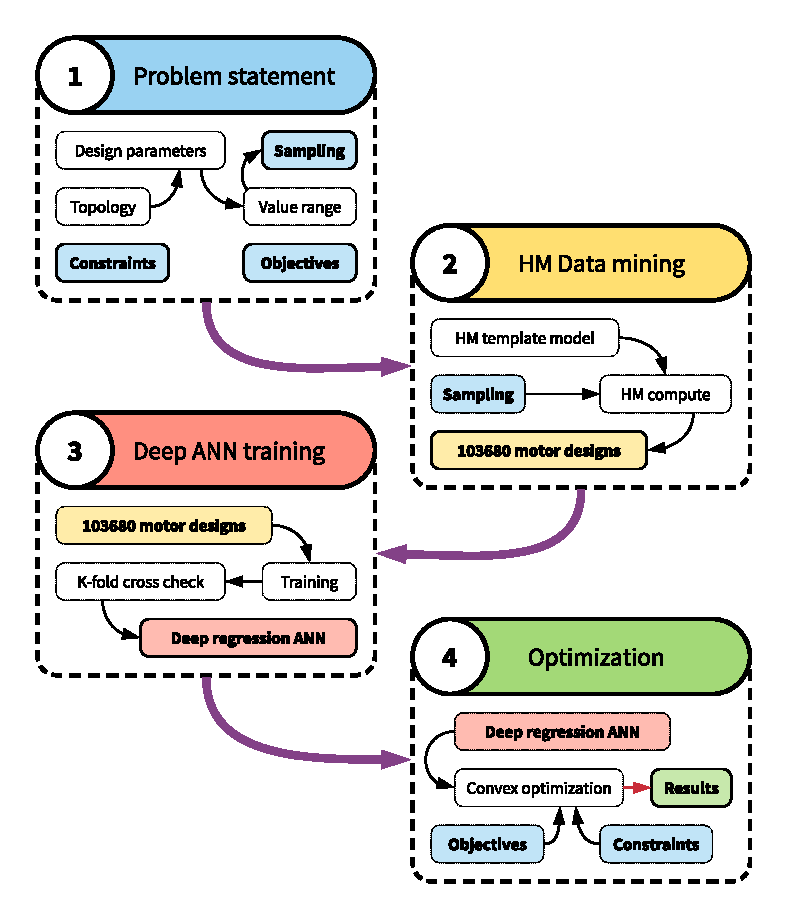
\includegraphics[width=4.5in]{chap4/images/optimization_process_RSM_for_PMLSM.pdf}
            \caption{Flowchart of the RSM motor design process adapted for PMLSM.}
            \label{fig:chapter/rsm/PMLSM optimization}
        \end{figure*}
        
        
        % -----------------------------------------------------------------------------------
        % --- NEW SUB SECTION --- NEW SUB SECTION --- NEW SUB SECTION --- NEW SUB SECTION --- 
        % -----------------------------------------------------------------------------------
        \subsection{Specifications \& Samplings}    \label{Chapter:RSM/PMLSM/spec}
        
        
            Reusing the considerations of the \acs{PMLSM} topology already presented in Section\,\ref{Chapter:PMLSM design HM/electromagnetic model/topology}, we refer to the design parameters $t_c$, $t_m$, $r_{mi}$, $L_k$, $\delta$ and their accompanying value ranges listed in Table\,\ref{table:table_of_optimization_constraints_PMLSM}. Additionally, $gap_{mc}$ and $gap_{cf}$ are addressed as constant values. 
            
            
            Table.\,\ref{table:RSM design level for PMLSM} shows incremental sampling steps for the structural design factors. From the sampling steps, full factorial design grid of $51840$ design were generated. Additional, the same number of design case constructed by random input variables in the ranges specified by Table\,\ref{table:RSM design level for PMLSM}. The purpose of combining the factorial design space and the randomly generated design cases is to help generalizing the supposedly continuous \acs{RSM} response better. In total, there were $103680$ independent motor designs available for \acs{ANN} training. To maximize the re-usability of the data collected, we choose to use \acs{HM} in order to generate a library of design for motors with only a single repeating unit. All of these motor designs are assumed to have the number of half coil periods $N_C$ and the number of half magnet periods $N_M$ of $1$. The input power will also be kept at $P=1500\mathrm{W}$, in order to directly compare with the study in Chapter\,\ref{Chapter:PMLSM design HM}.
            
            
            \begin{table}[!h]
                \renewcommand{\arraystretch}{1.2}
                \caption{Summary of motor parameter sampling levels for \acs{RSM} of \acs{PMLSM}}
                \label{table:RSM design level for PMLSM}
                \centering
                \begin{tabular}{@{}l r r r r r r r@{}}
                \hline
                \bfseries Params & \bfseries Level 1 & \bfseries Jump step & \bfseries Last level & \bfseries Unit \\
                \hline
                    $L_k$       &   18     &   2     &   90     &   $\mathrm{mm}$\\
                    $r_{mi}$    &    2     &   2     &   10     &   $\mathrm{mm}$\\
                    $t_m$       &    2     &   2     &   20     &   $\mathrm{mm}$\\
                    $t_c$       &    3     &   2     &   19     &   $\mathrm{mm}$\\
                    $\delta$    &  0.1     & 0.1     &  0.6     &   \\
                \hline
                \end{tabular}
            \end{table}
        
        
        % -----------------------------------------------------------------------------------
        % --- NEW SUB SECTION --- NEW SUB SECTION --- NEW SUB SECTION --- NEW SUB SECTION --- 
        % -----------------------------------------------------------------------------------
        \subsection{\acs{HM} data mining}           \label{Chapter:RSM/PMLSM/data mining}
        
        
            The base \acs{HM} computation model in Section\,\ref{Chapter:PMLSM design HM/electromagnetic model/hm solution} is re-purposed to help generate motor design data. To facilitate for the data mining and the optimization process later on, the same electromagnetic model was converted into a reusable function as illustrated in Fig.\,\ref{fig:chapter/rsm/PMLSM/mining process}. The free inputs include the repeat length $L_k$, the inner radius of the cylindrical magnet array $r_mi$, the magnet radial thickness $t_m$, the coil radial thickness $t_c$, and the proportion of the radially magnetized magnet against the total length of the magnet. The fixed input includes the number of half coil-phase $N_C$, the number of half magnet-phase $N_M$, and the power $P$. On the output side, the data mining function provides the half repeating unit mass $M$, motor constant $K_m$ and the linear force produced $F$.
        
        
            \begin{figure}
                \centering
                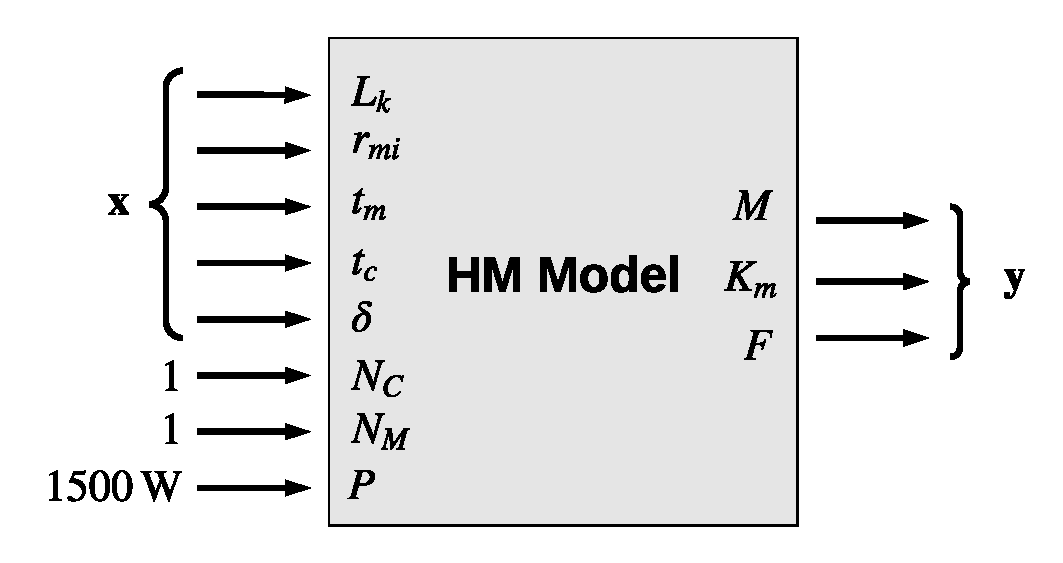
\includegraphics[width=4in]{chap4/images/HM_mining_for_PMLSM.pdf}
                \caption{A reusable function to obtain \acs{RSM} training data based on \ac{HM} calculations of \ac{PMLSM}.}
                \label{fig:chapter/rsm/PMLSM/mining process}
            \end{figure}
            
            
            The $103680$ input files through the reusable function as illustrated in Fig.\,\ref{fig:chapter/rsm/PMLSM/mining process} to obtain the corresponding outputs for each input set. The necessary information was then reduced back to a table that captured the motor design parameters in CSV format. 
            
        
        % -----------------------------------------------------------------------------------
        % --- NEW SUB SECTION --- NEW SUB SECTION --- NEW SUB SECTION --- NEW SUB SECTION --- 
        % -----------------------------------------------------------------------------------
        \subsection{Deep regression ANN training}   \label{Chapter:RSM/PMLSM/ANN training}
        
            
            Deep learning belongs to a broader family of machine learning methods and provides the most value in capturing complex non-linear patterns with almost any data set. The data set provides both the continuous input variables (structural design factors), and the continuous output variable (thrust characteristics at a given power), which classify our application as a supervised and regression type of machine learning problem.
            
            
            Since some design parameters ($gap_{mc}$, $gap_{cf}$, $P$ and others) were always established with constant values, the \acs{ANN} do not need to include them into the Input Layer. On the other hand, including both the thrust $F$ and the motor constant $K_m$ will introduce unwanted redundancy for a fixed power $P$ study. Three \acs{ANN} models were implemented and train using Keras and Tensorflow frameworks:
            
            
            \begin{itemize}
                \item $5$ structural parameters are regarded as the Input Layer: $L_k$,$r_{mi}$, $t_m$, $t_c$, and $\delta$,
                \item $1$ performance output is regarded as the Output Layer: $K_m$,
                \item The optimizer for training the \acs{ANN} is the Adam optimizer,
                \item $6$ hidden layers of densely connected nodes: $256-512-512-512-512-512$ for each layers
                \item Rectified linear unit (ReLU) activation function is used
for the input and hidden layer,
                \item Linear activation function is used for the output layer,
                \item The error to optimize for is \acs{MSE},
                \item The training and validation split chosen at random for each of the three models are: $70\%-30\%$, $75\%-25\%$, and $80\%-20\%$,
                The final \acs{ANN} model is ensembled from the average of three models above.
            \end{itemize}
            
            
            \begin{figure*}[!ht]
                \centering
                \subfloat[$70\%-30\%$ split model
                ]{
                    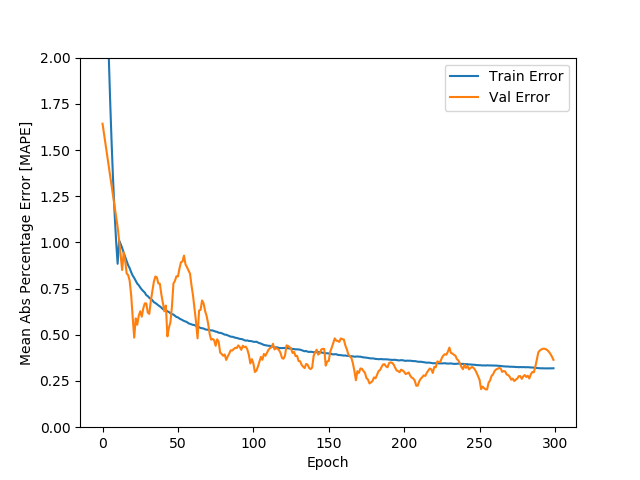
\includegraphics[width=0.5\textwidth]{chap4/images/MAPE_MSE_6_70-30_SPLIT.png}
                    \label{fig:chapter/rsm/PMLSM/training result/MAPE_70_30}
                }
                \subfloat[$75\%-25\%$ split model
                ]{
                    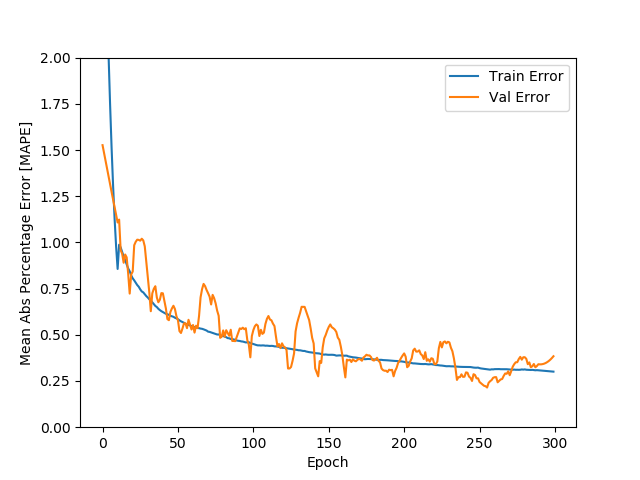
\includegraphics[width=0.5\textwidth]{chap4/images/MAPE_MSE_6_75-25_SPLIT.png}
                    \label{fig:chapter/rsm/PMLSM/training result/MAPE_75_25}
                }
                \\
                \subfloat[$80\%-20\%$ split model
                ]{
                    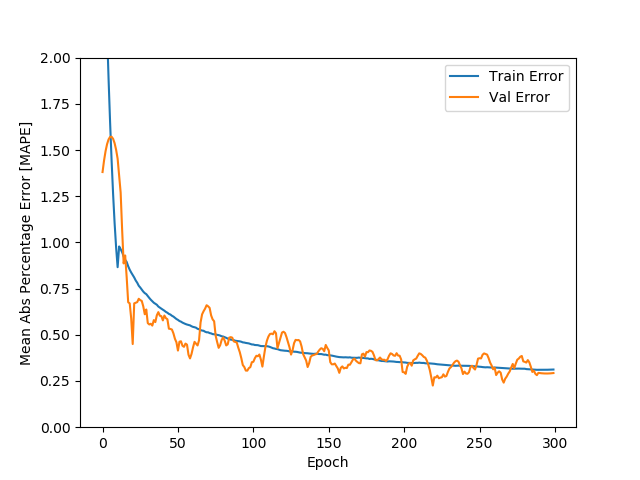
\includegraphics[width=0.5\textwidth]{chap4/images/MAPE_MSE_6_80-20_SPLIT.png}
                    \label{fig:chapter/rsm/PMLSM/training result/MAPE_80_20}
                }
                \caption{
                    Error produced by the deep learning \acs{ANN} model to represent \acsp{PMLSM}  vs. iterations for the training data (blue) and validation data (orange). The \acs{MAPE} is plotted for the training process of (a) $70\%-30\%$, (b) $75\%-25\%$, and (c) $80\%-20\%$ models, respectively.
                }   \label{fig:chapter/rsm/PMLSM/training result}
            \end{figure*}
            
            
            After $300$ training iteration, the models were shown to have an average \acf{MAPE} of $0.24\%$. The training and validation errors were similar, showing that the deep regression model is not over-fitted to the training data set. Fig.\,\ref{fig:chapter/rsm/PMLSM/training result} shows the training and validation error during the \acs{ANN} training process for each of the three models studied.
            
        
        % -----------------------------------------------------------------------------------
        % --- NEW SUB SECTION --- NEW SUB SECTION --- NEW SUB SECTION --- NEW SUB SECTION --- 
        % -----------------------------------------------------------------------------------
        \subsection{Optimization}                   \label{Chapter:RSM/PMLSM/Optimization}
        
        
            Following the outer and inner optimization setup in Section\,\ref{Chapter:PMLSM design HM/design optimization/optimization formulation}, this section repeat the optimization run with some differences. Instead of the \acs{HM} equations, the \acs{ANN} was employed to estimate the motor constant $K_m$ of a single repeat unit consisting of one half coil-phase ($N_C = 1$), and one half magnet-phase ($N_M = 1$). 
            
            
            During the execution of the optimization algorithm, many motors with half coil-phase values larger than $N_C = 1$ will be calculated. As mentioned previously, the \acs{ANN} only estimate $K_m$ for motor unit with $N_C=1$ and $N_M=1$. There requires a conversion for the motor constant of the whole motor $K_{m-whole}$, given that a new number of half coil-phase $N_{C-whole}$ that is larger than $1$:
            
            
            \begin{equation}
                K_{m-whole}=K_m  \sqrt{N_{C-whole}}
                \label{eq:calculate new K_m based on new N_C}
            \end{equation}
            
            
            Adapting to this change, the maximum jet velocity $v_{jet}$ becomes:
            
            
            \begin{equation}
                v_{jet} = \sqrt[4]{\frac{4P {K_{m-whole}}^2 {L_S}^2}{\rho_w V^2}}
                \label{eq:calculate new v_jet based on new N_C}
            \end{equation}
            
            
            Except when it comes to collecting the motor mass $M$, Equation\,\ref{eq:mass of motor via mass dimless} was borrowed from the \acs{HM} electromagnetic calculation. 
            
            
            \begin{figure*}[!ht]
                \par\bigskip
                \centering
                \subfloat[Sub-routine setup: Each objective function evaluation will start a separate sub-routine, taking about $6$ seconds.]{
                    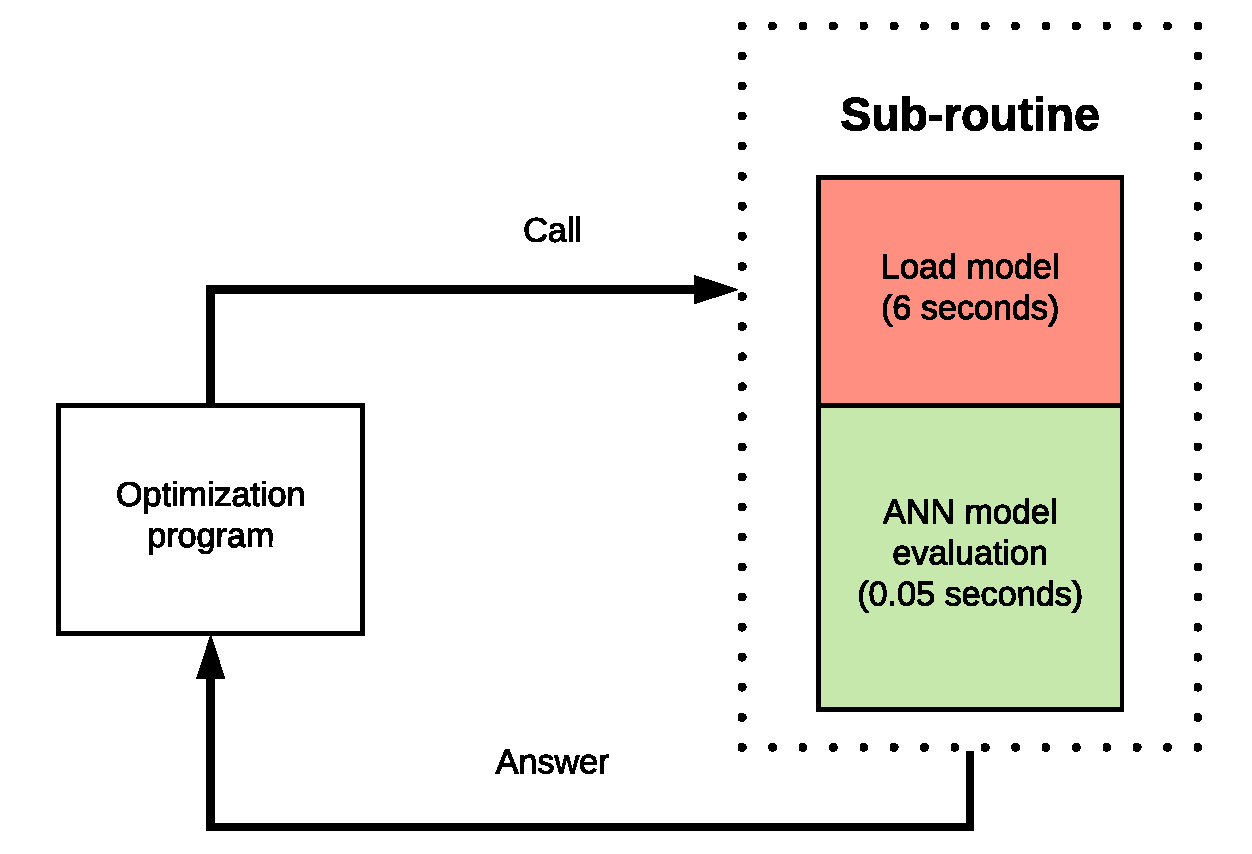
\includegraphics[width=0.45\textwidth]{chap4/images/inference_routine.pdf}
                    \label{fig:chapter/rsm/PMLSM/inference options/routine}
                }
                \,\,\,\,\,\,
                \subfloat[Web-server setup: The model is loaded only once, and all objective function evaluation takes less than $0.05$ seconds.]{
                    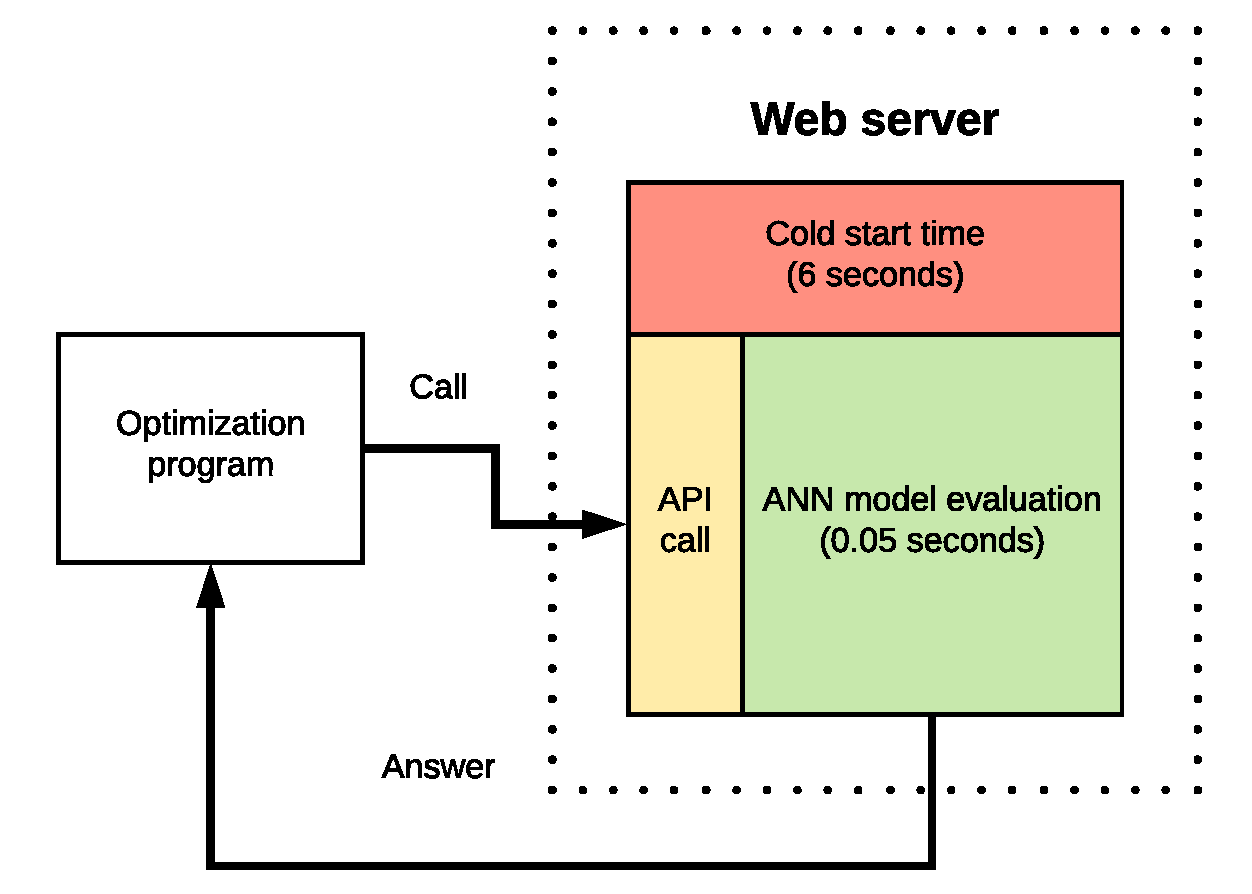
\includegraphics[width=0.45\textwidth]{chap4/images/inference_web_services.pdf}
                    \label{fig:chapter/rsm/PMLSM/inference options/web services}
                }
                \caption{
                    Two different style of optimization objective function evaluation.
                }\label{fig:chapter/rsm/PMLSM/inference options}
            \end{figure*}
            
            
            In the normal circumstance, a full execution cycle for inferring the \acs{ANN} model includes waiting for the model to load, querying the model, then terminating the model until the next execution. However, loading the \acs{ANN} model in Python environment may take a few seconds, the result is that numerous inferences of the existing model made by the optimization algorithm would cost an enormous amount of time. Alternatively, the optimization objective function evaluation should interact with the trained \acs{ANN} model in the fashion of a web server instead of a sub-routine, as illustrated in Fig.\,\ref{fig:chapter/rsm/PMLSM/inference options}


        % -----------------------------------------------------------------------------------
        % --- NEW SUB SECTION --- NEW SUB SECTION --- NEW SUB SECTION --- NEW SUB SECTION --- 
        % -----------------------------------------------------------------------------------
        \subsection{Results}                   \label{Chapter:RSM/PMLSM/Results}


            With the objective function evaluation using \acs{ANN} models at its core, the global optimization of \acs{PMLSM} for the problem described in Equation\,\ref{eq:outer optimization for PMLSMs} is summarized in Table\,\ref{table:result for global optimization of PMLSM via RSM method}. The table shows the optimization results for different motor mass constraints $M_0=[325,350,375,400,425]\,\mathrm{g}$.
            
            
            For instance, the global optimization of constraints set $P=1500\,\mathrm{W}$, $V=1\,\mathrm{mL}$, $gap_{mc}=1.2\,\mathrm{mm}$, $gap_{cf}=0.1\,\mathrm{mm}$, $M_0=325\,\mathrm{g}$ on the search space of $L_{M0}:120\,\mathrm{mm}\rightarrow 160\,\mathrm{mm}$, and $L_{C0}:50\,\mathrm{mm}\rightarrow 90\,\mathrm{mm}$, we found an under-hung motor with $N_C=4$, $N_M=12$, $L_k=26.5\,\mathrm{mm}$, $r_{mi}=2\,\mathrm{mm}$, $t_m=6.15\,\mathrm{mm}$, $t_c=3\,\mathrm{mm}$, $\delta=0.30$. The motor is able to theoretically produce $246.45\,\mathrm{N}$ at the rated power, which corresponds to a motor constant $K_m=6.36\,\mathrm{N/\sqrt{W}}$ and peak jet speed $v_{jet}=228.67\,\mathrm{m/s}$. Table\,\ref{table:result for global optimization of PMLSM via HM method} shows that same optimization problem powered by \acs{HM} electromagnetic equations produced almost exactly the same results when compared with \acs{RSM} method. The \acs{RSM} method predicted the peak jet speed $v_{jet}=228.67\,\mathrm{mm}$ while the \acs{HM} method predicted $v_{jet}=228.92\,\mathrm{mm}$. The only difference was the value of the ratio $\delta$ which does not affect the motor mass $M$.  
            
            
            Fig.\,\ref{fig:chapter/rsm/PMLSM/results} provides global optimization plots of $v_{jet}$ for the search space $L_{M0}:120\,\mathrm{mm}\rightarrow 160\,\mathrm{mm} \times L_{C0}:50\,\mathrm{mm}\rightarrow 90\,\mathrm{mm}$ using $P=1500\,\mathrm{W}$, $V=1\,\mathrm{mL}$, $gap_{mc}=1.2\,\mathrm{mm}$, $gap_{cf}=0.1\,\mathrm{mm}$,  and $M_0=[325,350,375,400,425]\,\mathrm{g}$. Not only the global optimization results obtained by different modelling methods agree strongly, the contour plots populated by the optimization processes of \acs{RSM} (Fig.\,\ref{fig:chapter/rsm/PMLSM/results}) and \acs{HM} (Fig.\,\ref{fig:chapter/hm/optimization search space result for differnt mass}) looked almost identical. This study has successfully demonstrated the effectiveness and accuracy of design and optimization process presented Section\,\ref{Chapter:RSM/outline}.
        

            
            \begin{landscape}
                \begin{table}
                    \renewcommand{\arraystretch}{1.2}
                    \caption{Summary of motor design optimization values and performance using \acs{RSM} method}
                    \label{table:result for global optimization of PMLSM via RSM method}
                    \centering
                    \begin{tabular}{lllrrrrr}
                        \hline
                        \textbf{Params}     & \textbf{Description}                            & \textbf{Unit}           & $M_0=\mathbf{325\,g}$ & $\mathbf{350\,g}$ & $\mathbf{375\,g}$ & $\mathbf{400\,g}$ & $\mathbf{425\,g}$ \\
                        \hline
                        $P$        & Power dissipation in coil winding      & $\mathrm{kW}$  & $1.50$                & $1.50$            & $1.50$            & $1.50$            & $1.50$            \\
                        $V$        & Volume of ampoule                      & $\mathrm{mL}$  & $1.00$                & $1.00$            & $1.00$            & $1.00$            & $1.00$            \\
                        $gap_{mc}$ & Magnet and coil fixed gap              & $\mathrm{mm}$  & $1.20$                & $1.20$            & $1.20$            & $1.20$            & $1.20$            \\
                        $gap_{cf}$ & Coil and iron fixed gap                & $\mathrm{mm}$  & $0.10$                & $0.10$            & $0.10$            & $0.10$            & $0.10$            \\
                        \hline
                        $L_{C0:optim}$ & Constraint $L_C$ winding at global optimum & $\mathrm{mm}$        & $53.00$                       & $53.00$           & $53.00$           & $53.00$           & $53.00$           \\
                        $L_{M0:optim}$ & Constraint $L_C+L_S$ at global optimum        & $\mathrm{mm}$        & $160.00$                      & $160.00$          & $160.00$          & $160.00$          & $160.00$          \\
                        \hline
                        $r_{mi}$   & Magnet array inner radius              & $\mathrm{mm}$  & $2.00$                & $2.00$            & $2.00$            & $2.00$            & $2.00$            \\
                        $t_m$      & Magnet thickness                       & $\mathrm{mm}$  & $6.15$                & $6.35$            & $6.67$            & $6.99$            & $7.29$            \\
                        $t_c$      & Coil thickness                         & $\mathrm{mm}$  & $3.00$                & $3.00$            & $3.00$            & $3.00$            & $3.00$            \\
                        $\delta$   & Ratio of radial magnet vs. magnet pair &                & $0.32$                & $0.25$            & $0.25$            & $0.25$            & $0.27$            \\
                        $N_C$      & Number of half coil-poles              &                & $4$                   & $3$               & $3$               & $3$               & $3$               \\
                        $N_M$      & Number of half magnet-poles            &                & $12$                  & $9$               & $9$               & $9$               & $9$               \\
                        \hline
                        $t_f$      & Iron shell thickness                   & $\mathrm{mm}$  & $0.77$                        & $1.07$            & $1.12$            & $1.15$            & $1.19$    \\       
                        $L_k$      & Full pole length                       & $\mathrm{mm}$  & $26.50$               & $35.33$           & $35.33$           & $35.33$           & $35.33$           \\
                        $L_C$      & Length of coil array                   & $\mathrm{mm}$  & $53.00$               & $53.00$           & $53.00$           & $53.00$           & $53.00$           \\
                        $L_M$      & Length of magnet array                 & $\mathrm{mm}$  & $159.00$              & $159.00$          & $159.00$          & $159.00$          & $159.00$          \\
                        $L_S$      & Stroke length                          & $\mathrm{mm}$  & $106.00$              & $106.00$          & $106.00$          & $106.00$          & $106.00$          \\
                        \hline
                        $v_{jet}$  & Achievable jet speed                   & $\mathrm{m/s}$ & $228.64$              & $234.21$          & $239.81$          & $245.13$          & $250.10$         \\
                        $F$        & Force exerts on piston                 & $\mathrm{N}$         & $246.45$                      & $258.72$          & $271.35$          & $283.44$          & $295.06$          \\
                        $K_m$      & Motor constant                         & $\mathrm{N/\sqrt{W}}$ & $6.36$                        & $6.68$            & $7.01$            & $7.32$            & $7.62$           \\
                        \hline
                    \end{tabular}
                \end{table}
            \end{landscape}
            
            \begin{figure*}[!ht]
                \centering
                \subfloat[$M_0=325\,\mathrm{g}$. Global optimum found at $L_{C0}=53\,\mathrm{mm}$, $L_{C0}=160\,\mathrm{mm}$, $N_C=4$, and $N_M=12$.
                ]{
                    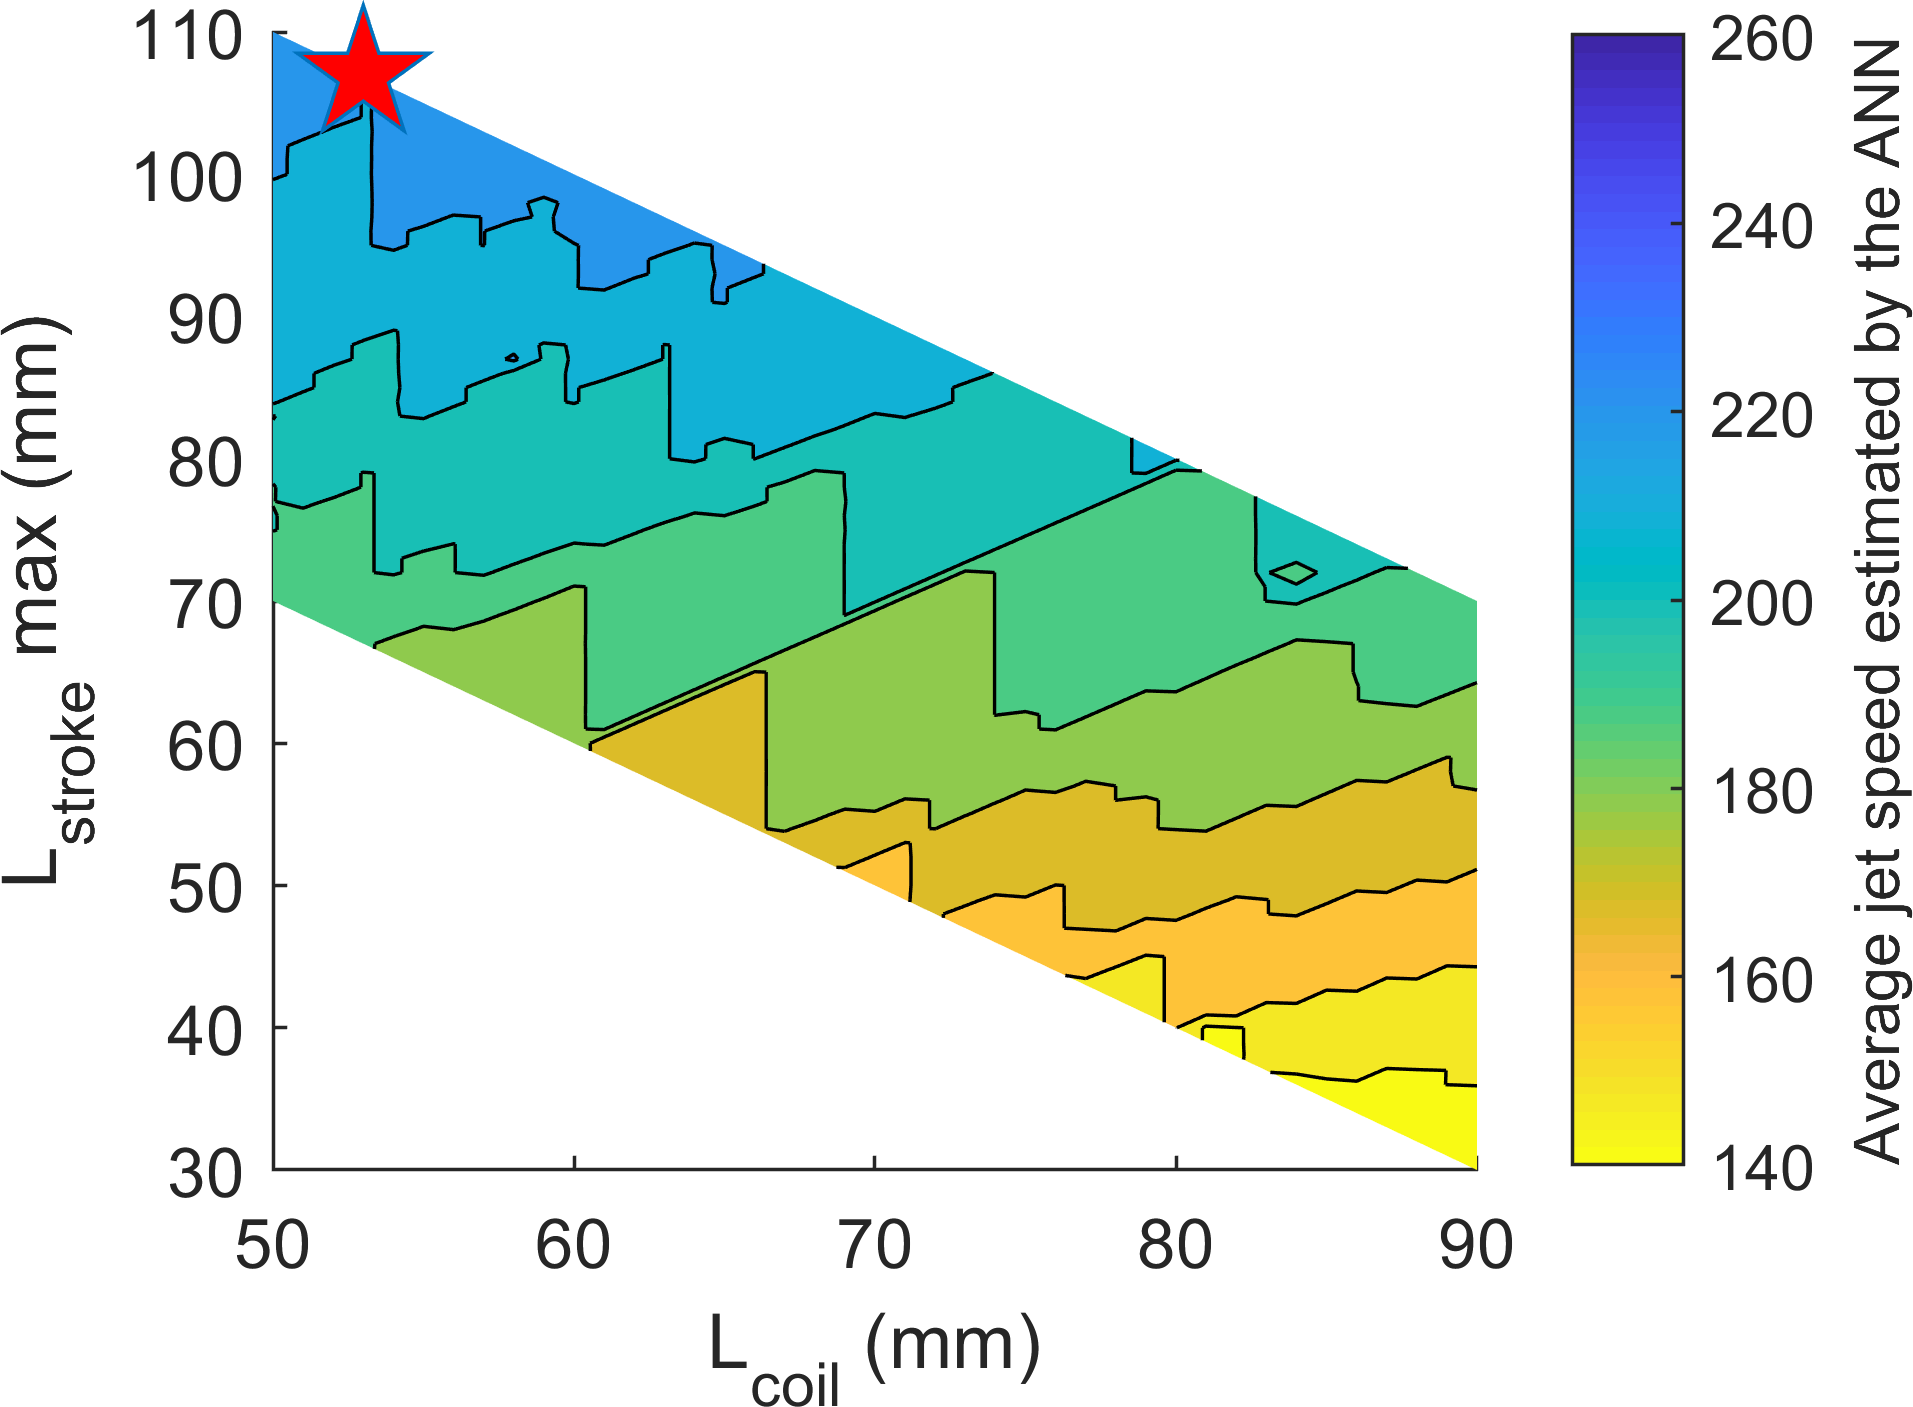
\includegraphics[width=0.45\textwidth]{chap4/images/PMLSM_RSM_325g.png}
                    \label{fig:chapter/rsm/PMLSM/results/325}
                }
                \qquad
                \subfloat[$M_0=350\,\mathrm{g}$ Global optimum found at $L_{C0}=53\,\mathrm{mm}$, $L_{C0}=160\,\mathrm{mm}$, $N_C=3$, and $N_M=9$.
                ]{
                    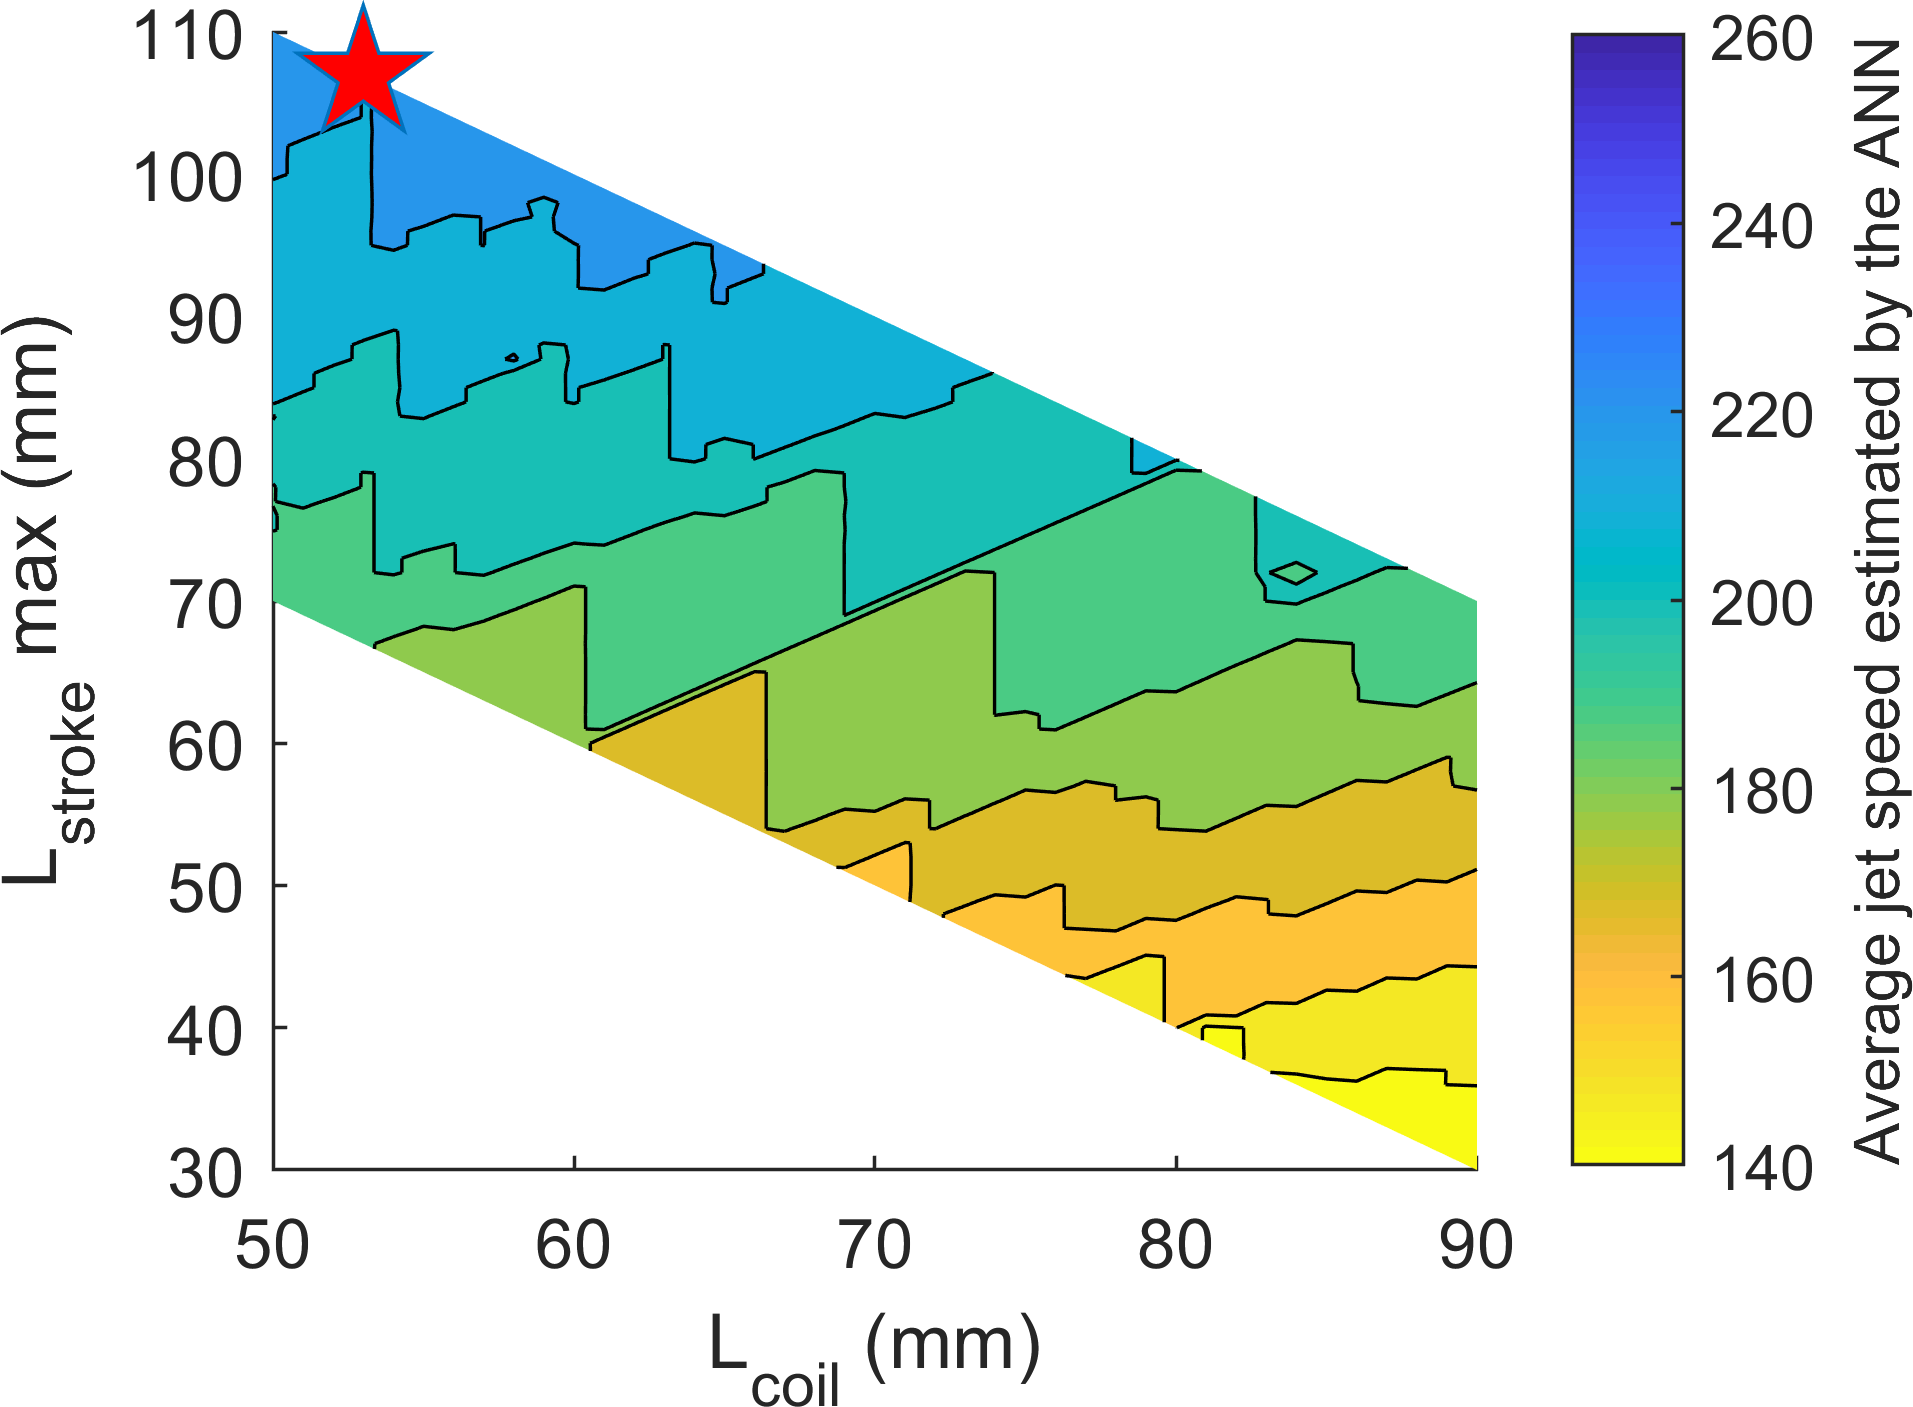
\includegraphics[width=0.45\textwidth]{chap4/images/PMLSM_RSM_325g.png}
                    \label{fig:chapter/rsm/PMLSM/results/350}
                }
                \\
                \subfloat[$M_0=375\,\mathrm{g}$. Global optimum found at $L_{C0}=53\,\mathrm{mm}$, $L_{C0}=160\,\mathrm{mm}$, $N_C=3$, and $N_M=9$.
                ]{
                    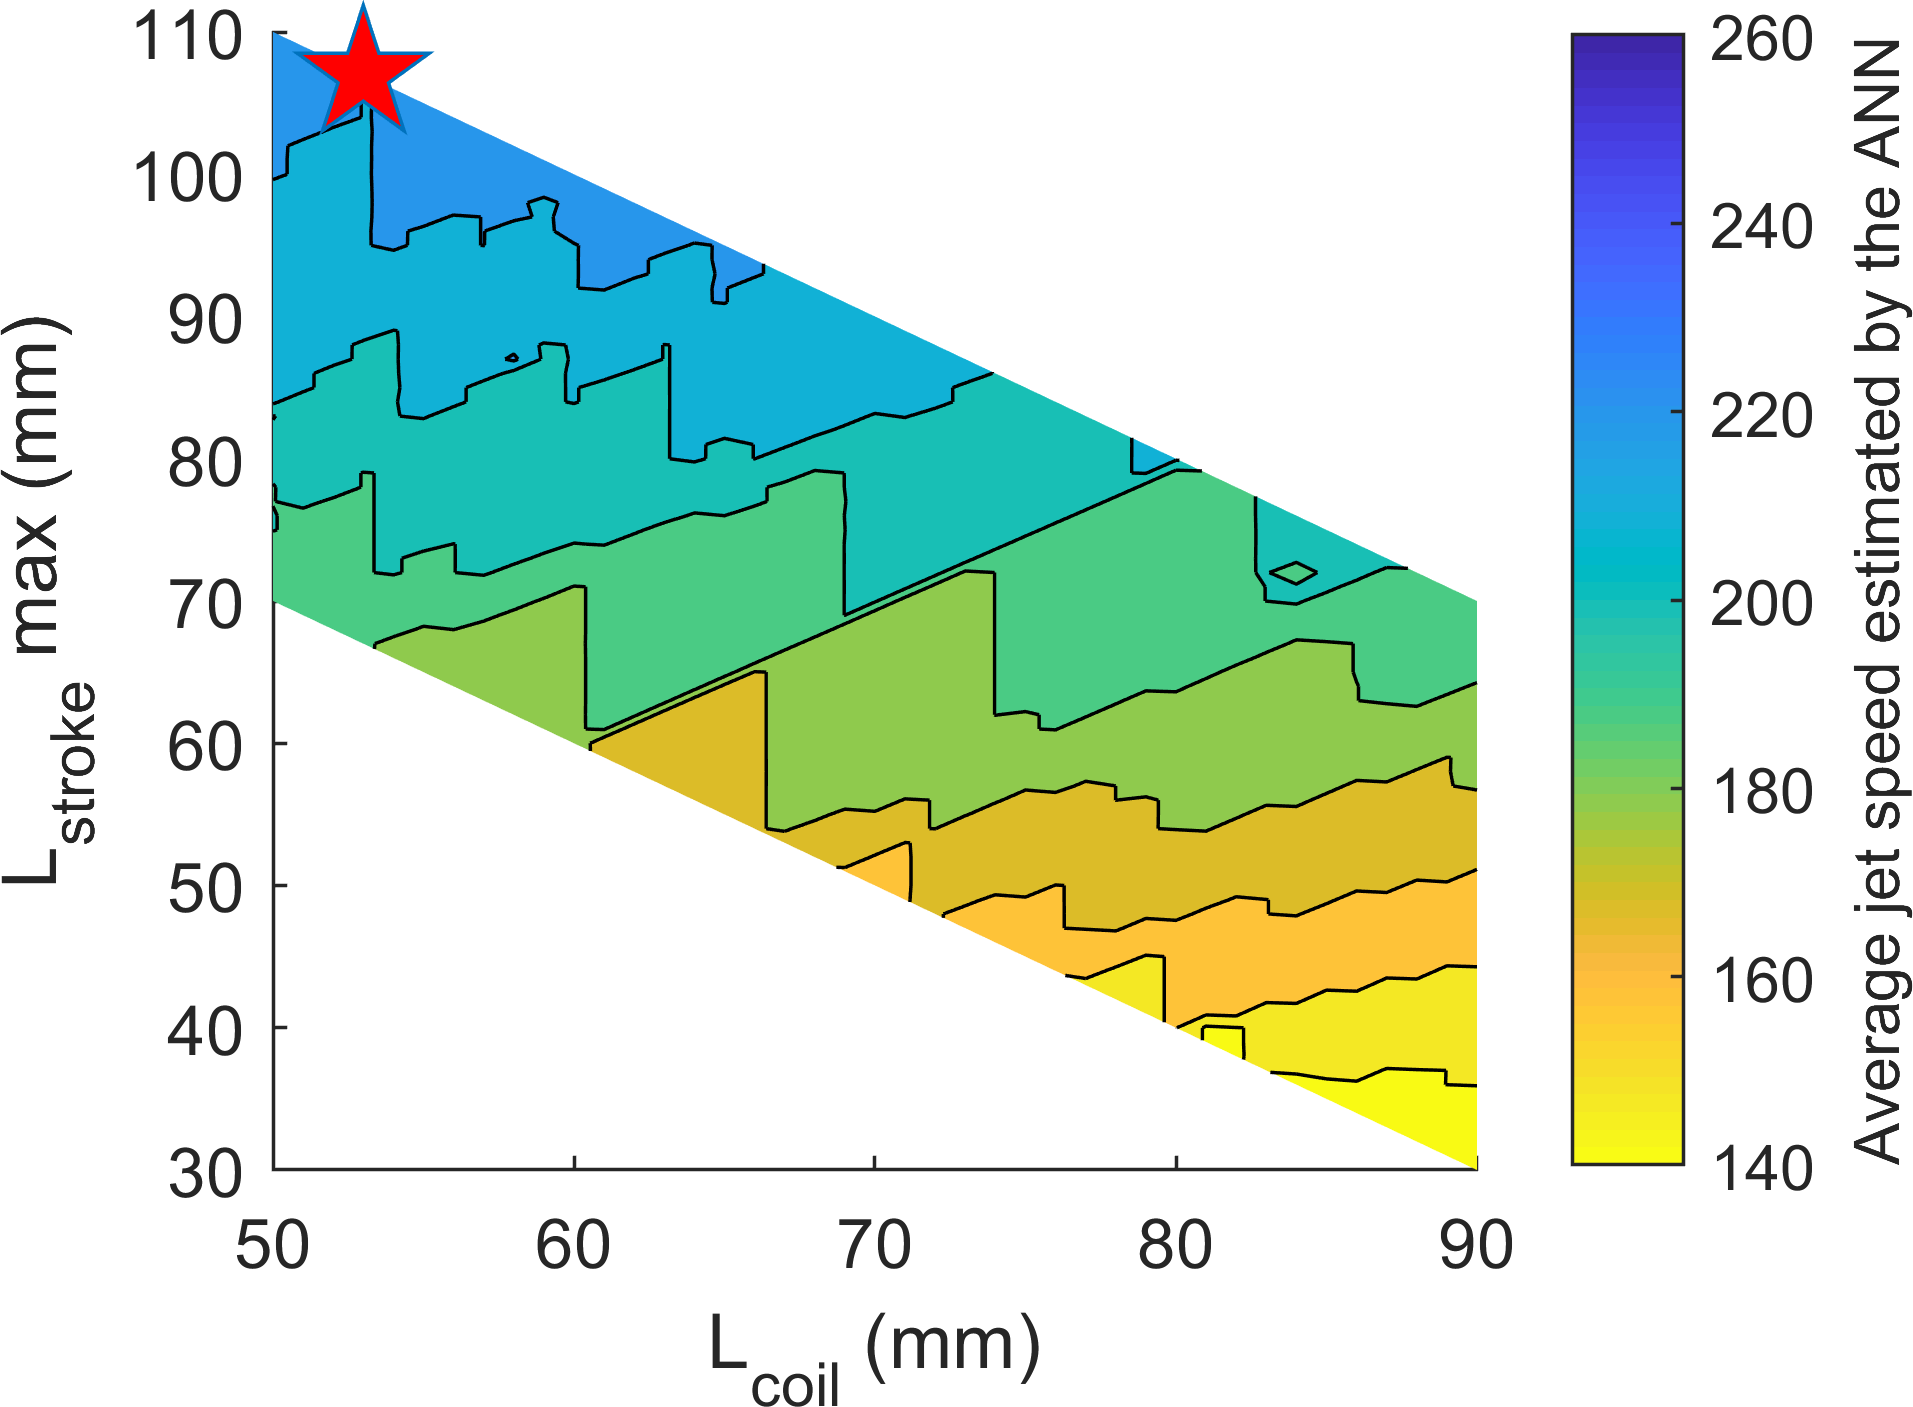
\includegraphics[width=0.45\textwidth]{chap4/images/PMLSM_RSM_325g.png}
                    \label{fig:chapter/rsm/PMLSM/results/375}
                }
                \qquad
                \subfloat[$M_0=400\,\mathrm{g}$. Global optimum found at $L_{C0}=53\,\mathrm{mm}$, $L_{C0}=160\,\mathrm{mm}$, $N_C=3$, and $N_M=9$.
                ]{
                    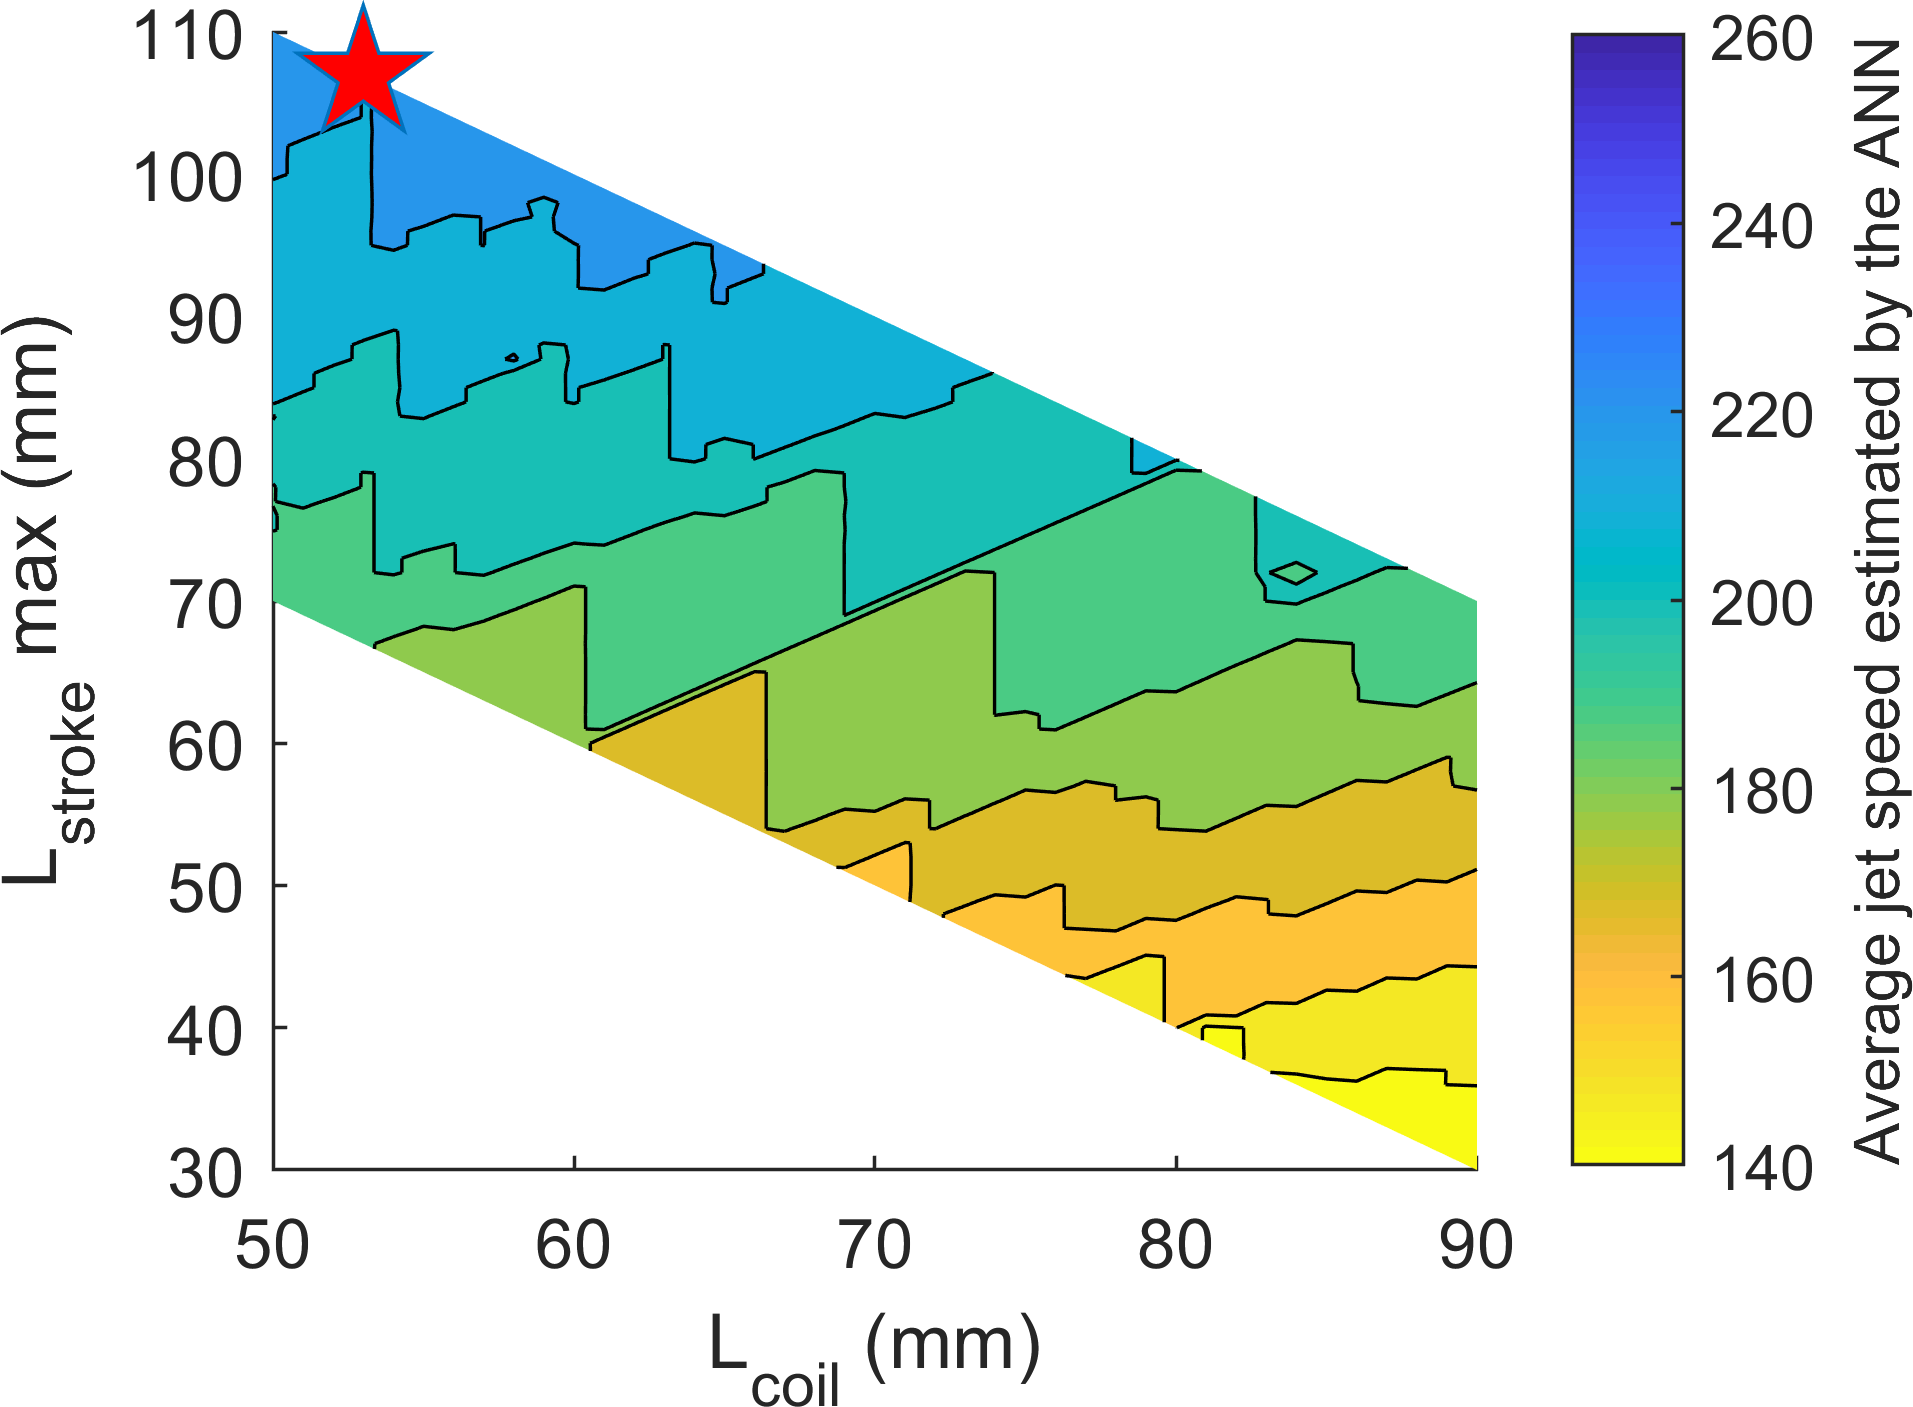
\includegraphics[width=0.45\textwidth]{chap4/images/PMLSM_RSM_325g.png}
                    \label{fig:chapter/rsm/PMLSM/results/400}
                }
                \\
                \subfloat[$M_0=425\,\mathrm{g}$. Global optimum found at $L_{C0}=53\,\mathrm{mm}$, $L_{C0}=160\,\mathrm{mm}$, $N_C=3$, and $N_M=9$.
                ]{
                    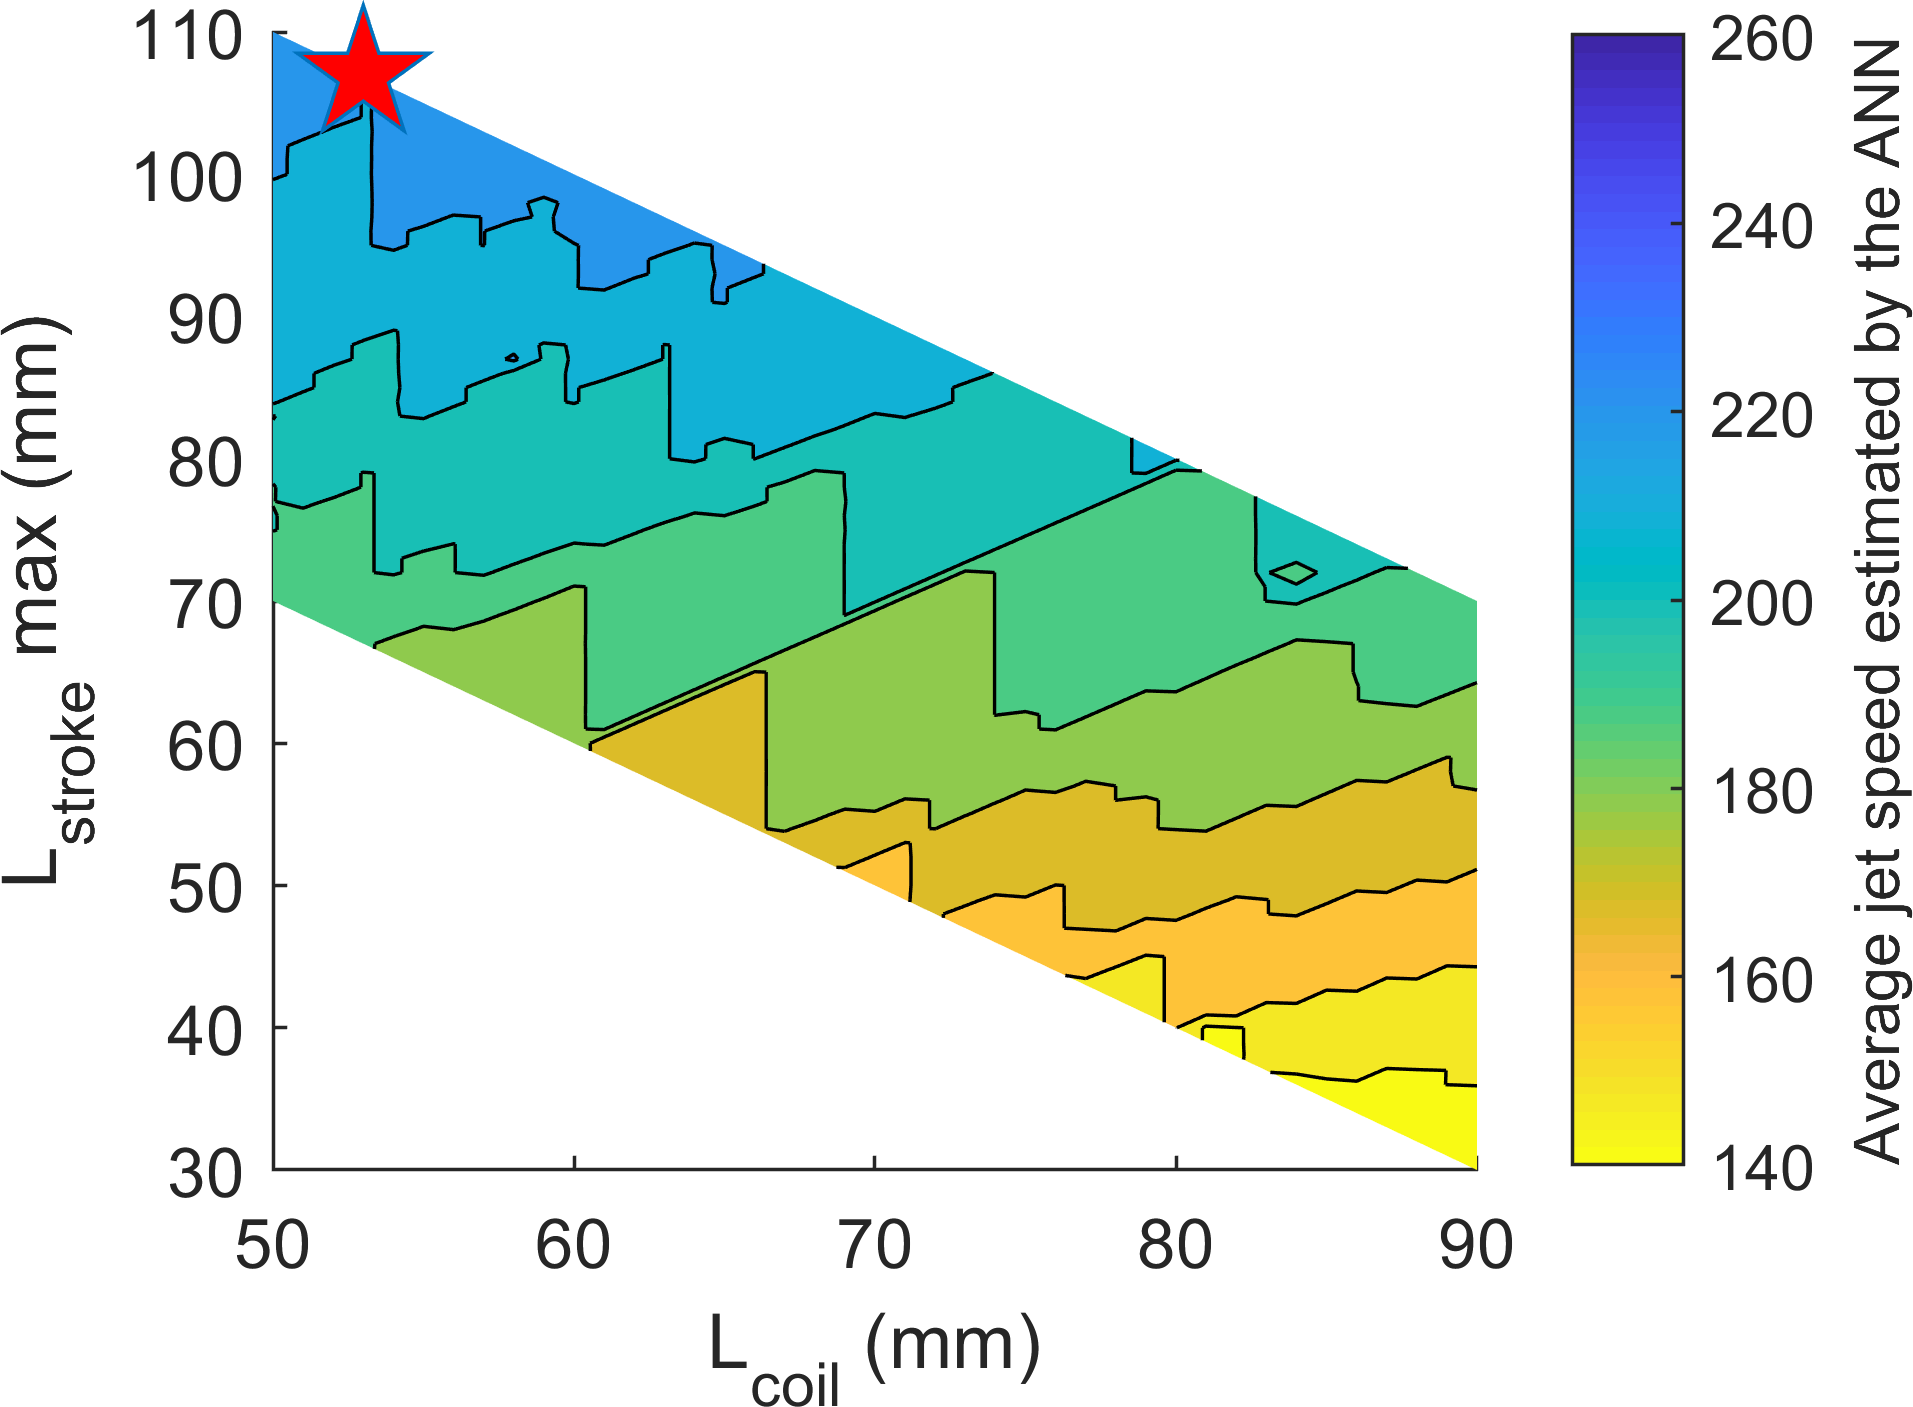
\includegraphics[width=0.45\textwidth]{chap4/images/PMLSM_RSM_325g.png}
                    \label{fig:chapter/rsm/PMLSM/results/425}
                }
                \\
                \caption{
                    The global optimization plots of $v_{jet}$ for the search space $L_{M0}:120\,\mathrm{mm}\rightarrow 160\,\mathrm{mm} \times L_{C0}:50\,\mathrm{mm}\rightarrow 90\,\mathrm{mm}$ using $P=1500\,\mathrm{W}$, $V=1\,\mathrm{mL}$, $gap_{mc}=1.2\,\mathrm{mm}$, $gap_{cf}=0.1\,\mathrm{mm}$,  and $M_0$ of: (a) $325\,\mathrm{g}$, (b) $350\,\mathrm{g}$, (c) $375\,\mathrm{g}$, (d) $400\,\mathrm{g}$, and (e) $425\,\mathrm{g}$.
                }   \label{fig:chapter/rsm/PMLSM/results}
            \end{figure*}
    
    % ===================================================================================================
    % === NEW SECTION === NEW SECTION === NEW SECTION === NEW SECTION === NEW SECTION === NEW SECTION ===
    % ===================================================================================================
    \section{Application to \ac{LFSM}}               \label{Chapter:RSM/LFSM}
    
    
        This study attempts to clarify the performance characteristics of \acsp{LFSM} when applied to \acs{NFJI} applications. We chose to examine a C-core topology, because they typically produce more thrust than E-core topologies \cite{Min2011OptimizationMachines}. A conventional 6 slot/5 pole \acs{LFSM} as shown in Fig.\,\ref{fig:chapter/rsm/LFSM/structure/6-5} has minimal thrust ripple due to cancellation of even order and third order harmonics. However, we chose to study a 6 slot/7 pole LFSM structure as illustrated  in Fig.\,\ref{fig:chapter/rsm/LFSM/structure/6-7} because it is reported to also produce more thrust than other configurations, even though it may come at the expense of having more thrust ripple \cite{Chen2010}. 
        
        
        \begin{figure*}[!ht]
            \centering
            \subfloat[\label{fig:chapter/rsm/LFSM/structure/6-7}Tubular LFSM with 6 slots and 7 poles per period.]{
                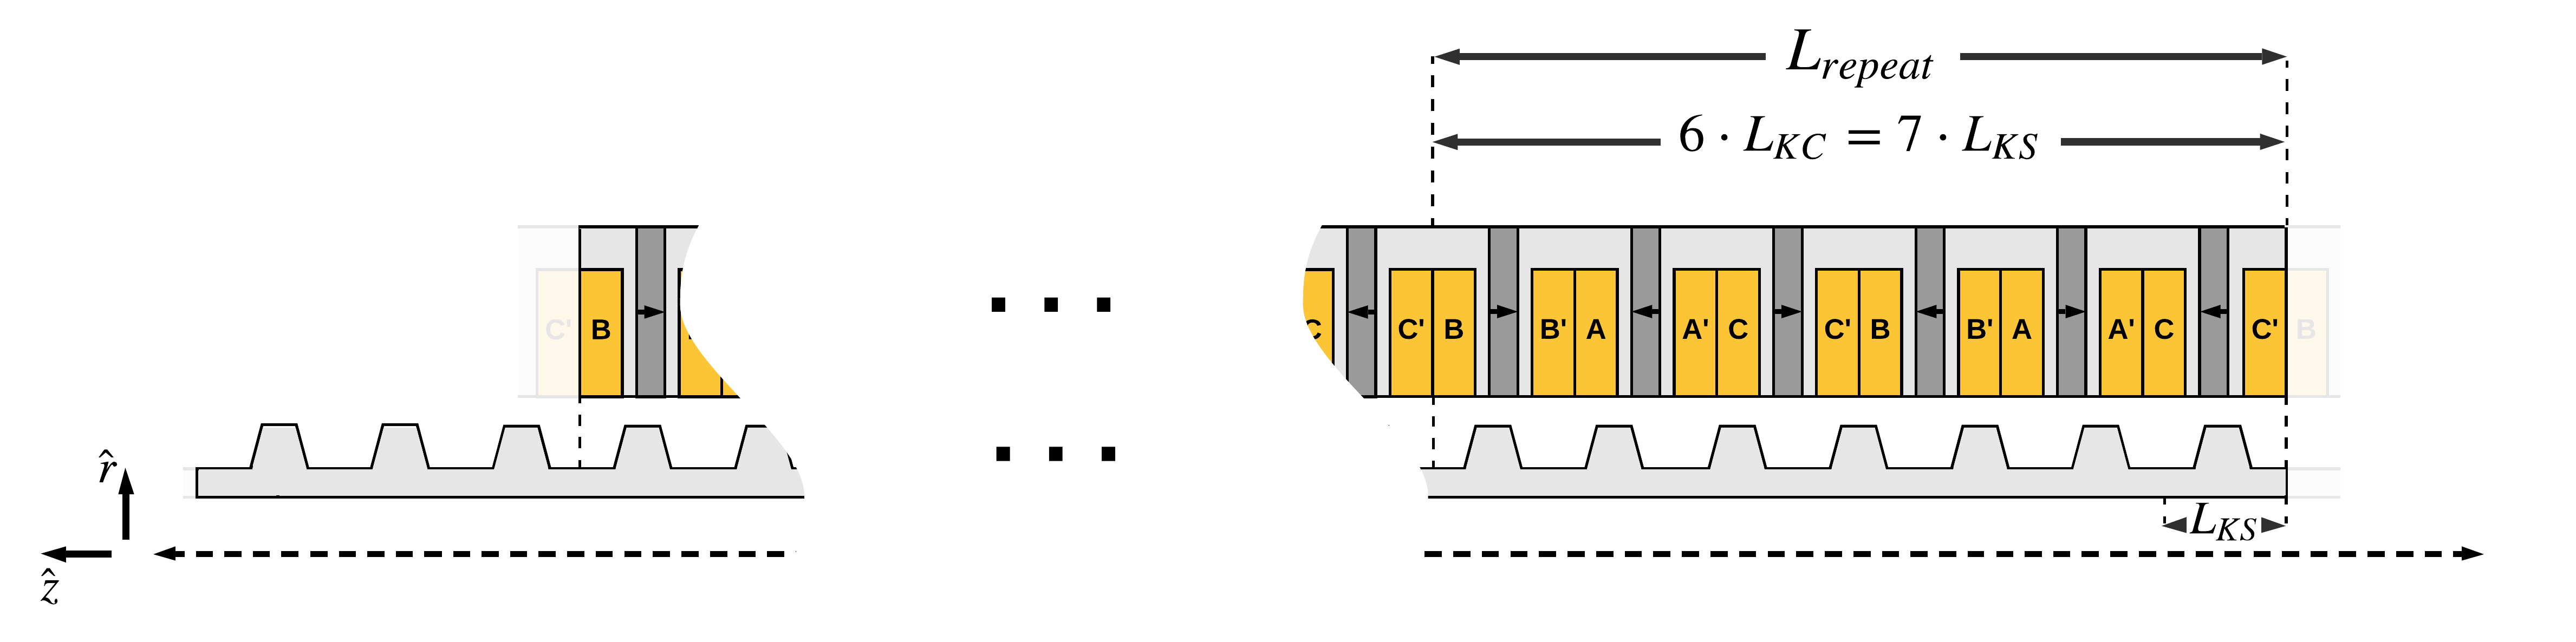
\includegraphics[width=0.97\textwidth]{chap4/images2/LFSM_6_7.png}
            }
            \\
            \subfloat[\label{fig:chapter/rsm/LFSM/structure/6-5}Tubular LFSM with 6 slots and 5 poles per period.]{
                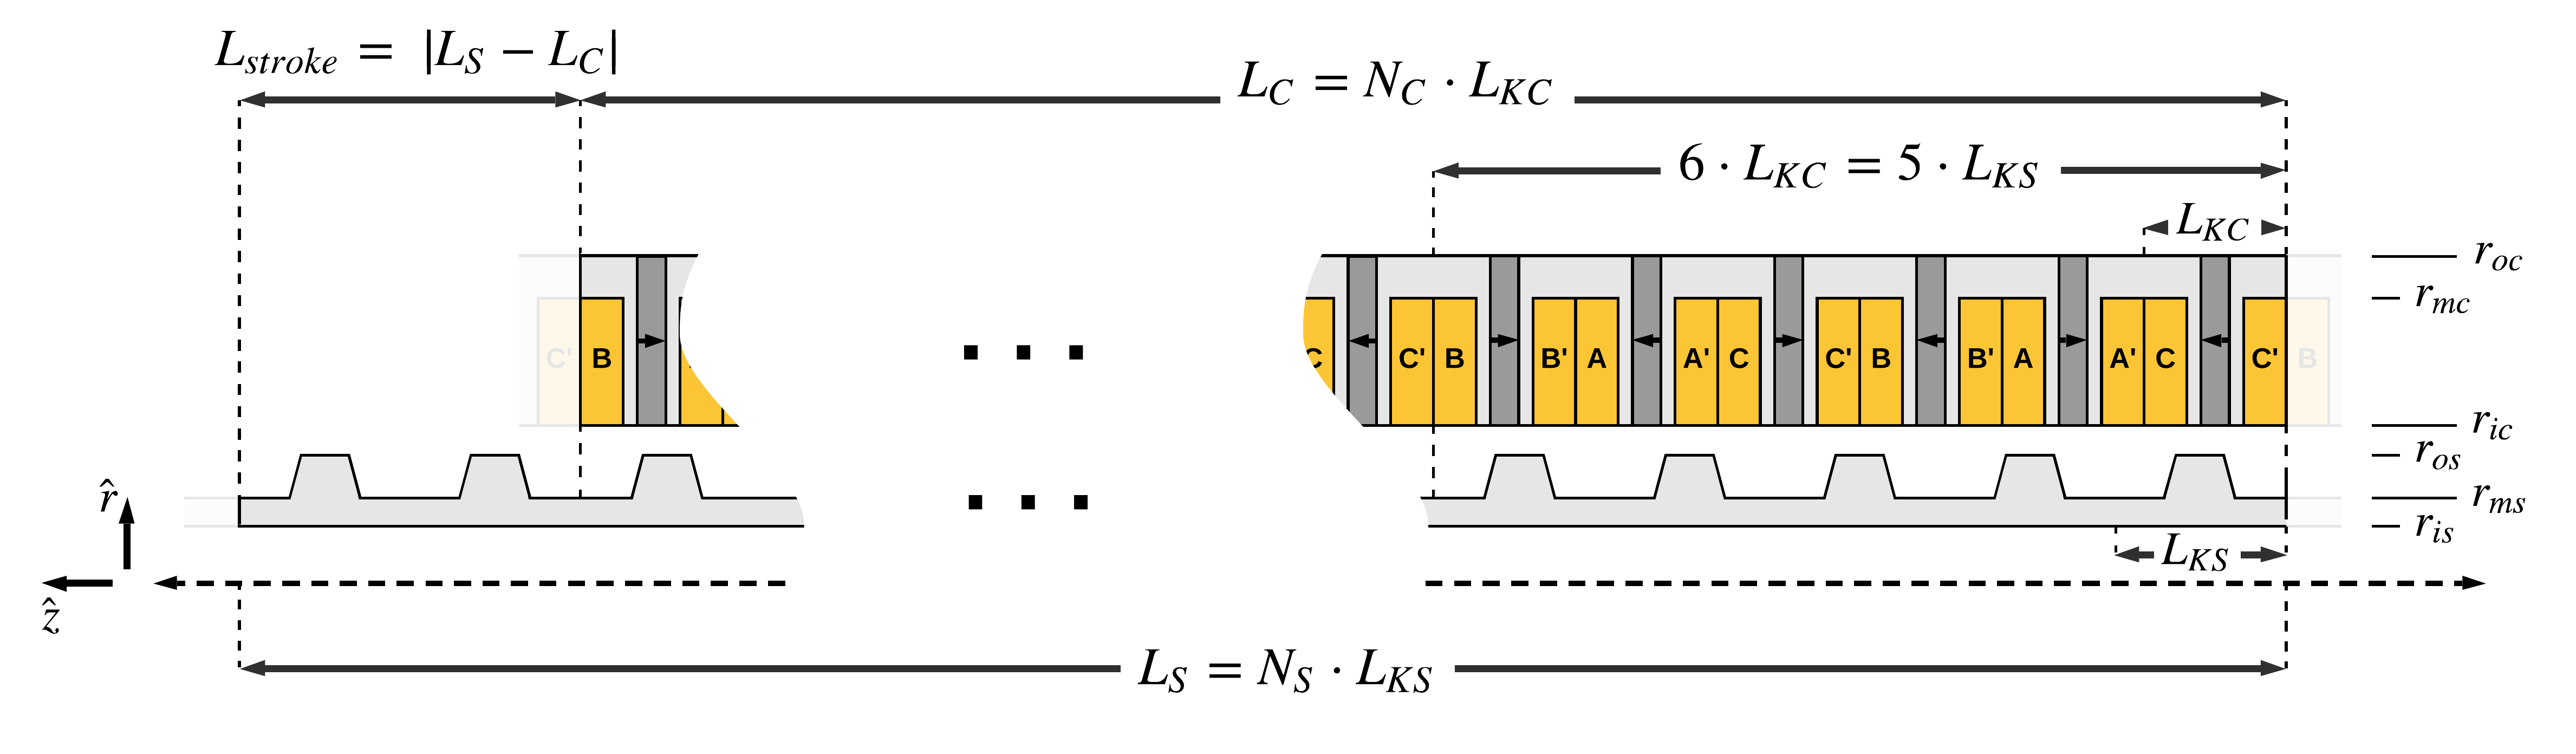
\includegraphics[width=0.97\textwidth]{chap4/images2/LFSM_6_5.png}
            }
            \caption{Schematic of tubular \acs{LFSM}
                \label{fig:conventional_flux_switching_machines}
            }\label{fig:chapter/rsm/LFSM/structure}
        \end{figure*}
        
        
        The general parameters of a three-phase tubular linear flux-switching motor consist of:
        
        \begin{itemize}
            \item The total number of armature slots $N_C$,
            \item The total number of armature pole $N_S$
            \item The radii of the \acs{SMC} track $r_{is}$, $r_{ms}$, and $r_{os}$,
            \item The radii of the armature assembly $r_{ic}$, $r_{mc}$, and $r_{oc}$,
            \item The slot period length $L_{KC}$,
            \item The track period length $L_{KS}$,
            \item The whole of mover armature length $L_{C}$,
            \item The whole track length or equivalent motor length $L_{S}$,
            \item The length of each overall repeat unit $L_{repeat}$,
            \item The motor stroke length $L_{stroke}$.
        \end{itemize}
        
        
        \begin{figure*}
            \centering
            \subfloat[\label{fig:chapter/rsm/LFSM/machine design/params} Detailed dimensions]{
                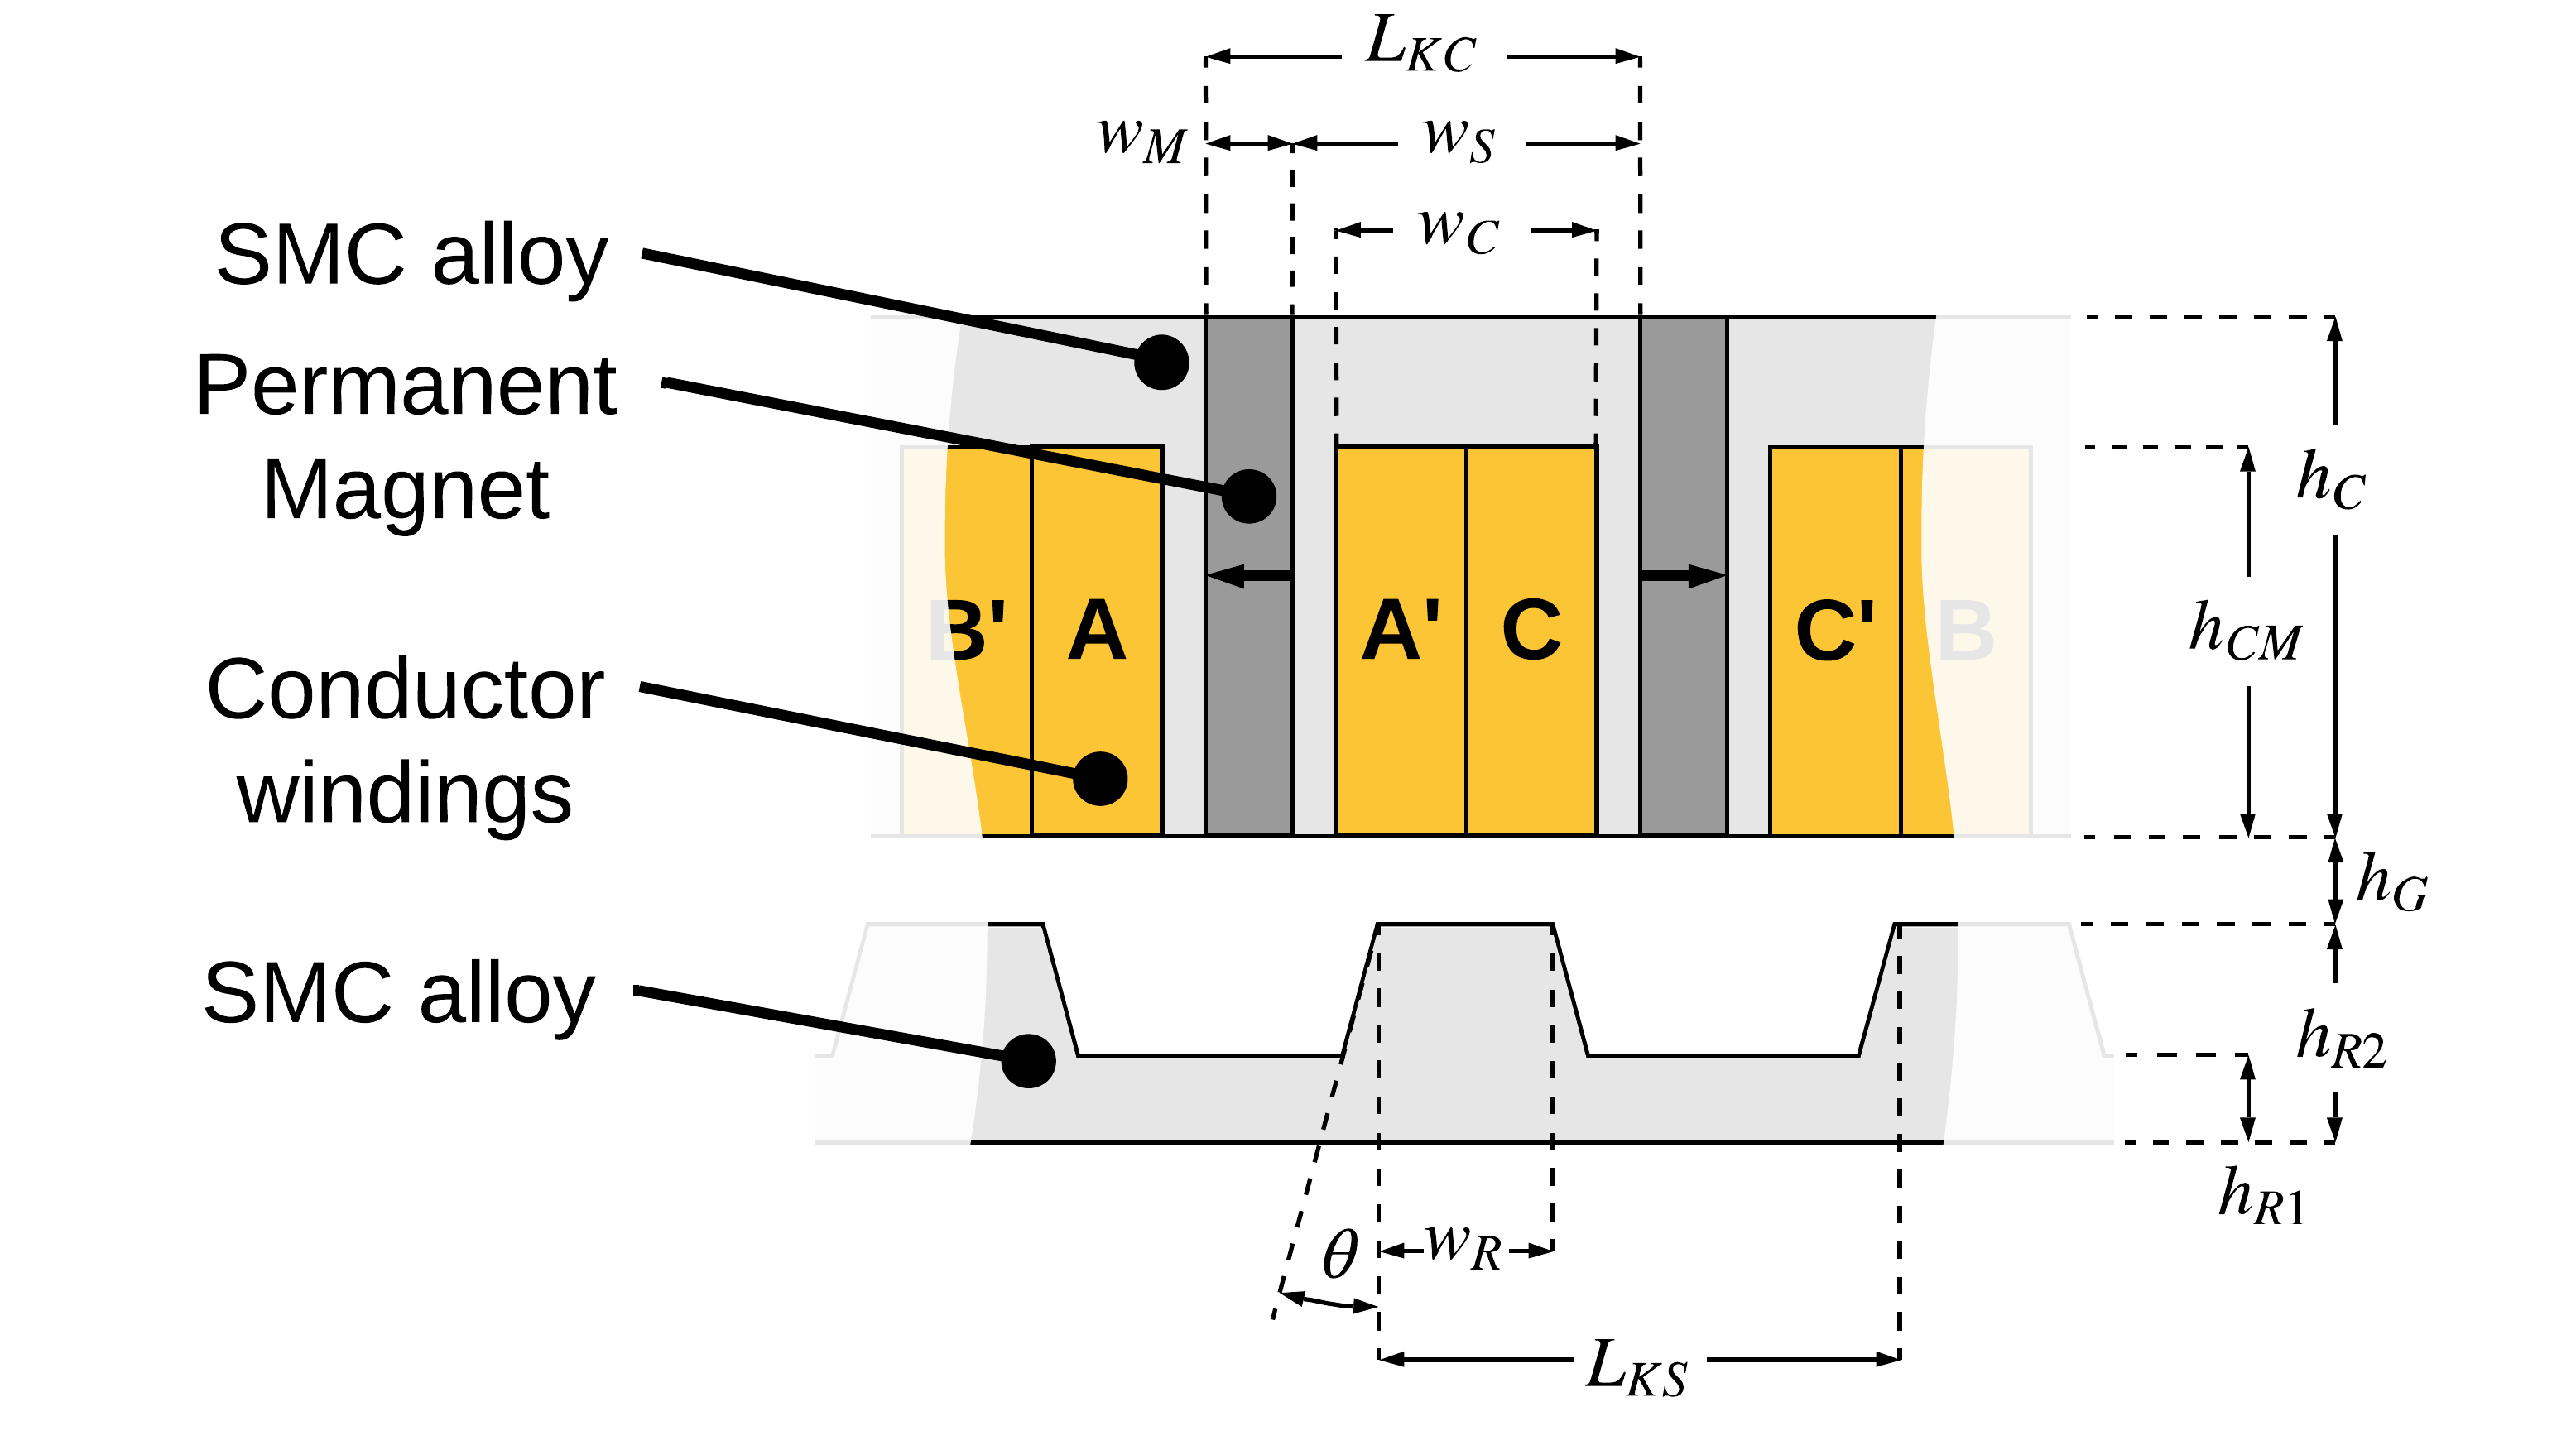
\includegraphics[width=0.7\textwidth]{chap4/images2/params.png}
            }
            \\
            \subfloat[\label{fig:chapter/rsm/LFSM/machine design/setup} A jet injector driven by a LFSM]{
                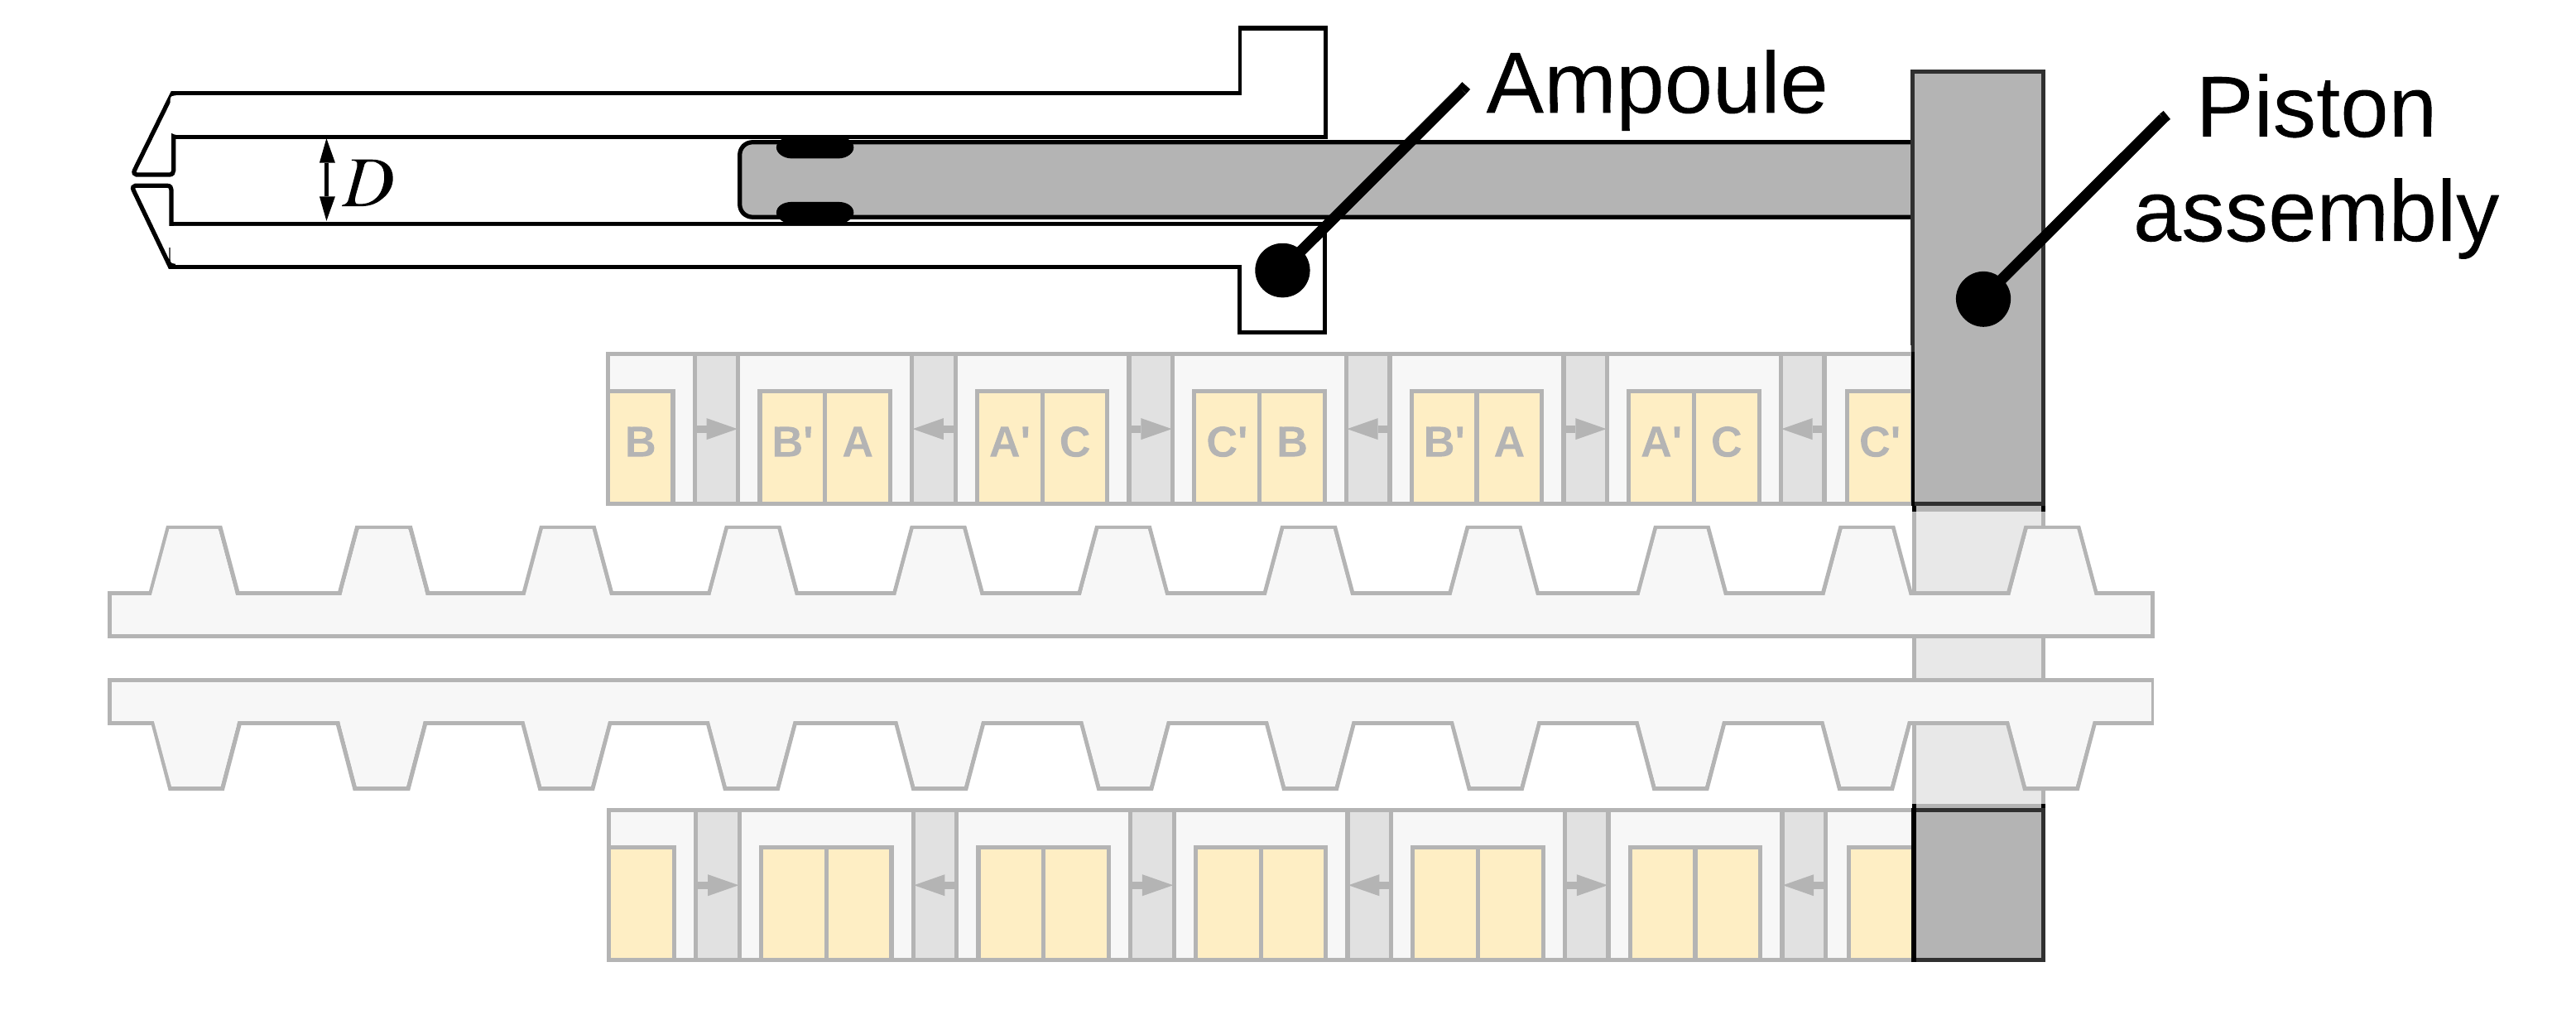
\includegraphics[width=0.8\textwidth]{chap4/images2/machine_setup.png}
            }
            \caption{ 
                \label{fig:chapter/rsm/LFSM/machine design}Detailed dimensions of the tubular LFSM: 
                armature assembly widths ($w_M$, $w_S$, $w_C$),
                armature assembly heights ($h_{CM}$, $h_{C}$),
                track tooth width ($w_{R}$),
                and track tooth heights ($h_{R1}$, $h_{R2}$), tooth angle $\theta$, air gap $h_G$ in $\mathrm{(a)}$. A basic schematic of a LFSM driven jet injector and a NFJI drug ampoule with diameter $D$ are shown in $\mathrm{(b)}$.
            }
        \end{figure*}
        
        
        To minimize the moving (and total) mass, the outer sliding armature assembly is selected as the moving element. Each repeating period of the motor consists of 6 axially magnetized permanent magnet rings, 6 \acf{SMC} cylindrical cores to contain the conductor windings, and 2 circumstantially wound three-phase coil groups. The secondary is passive, and constructed as an SMC tube with a periodic tooth structure with angled sides. Dimensions are shown for each topology in Fig.\,\ref{fig:chapter/rsm/LFSM/machine design/params}. Additionally, Fig.\,\ref{fig:chapter/rsm/LFSM/machine design/setup} illustrates how a tubular \acs{LFSM} can be incorporated in the design of a hand-held jet injector device.
        
        
        Additional design ratios were established to better capture the parametric representation of the 6 slot/7 pole tubular \acs{LFSM}:
        
        
        \begin{equation}
            \alpha=\frac{w_M}{L_{KC}}
            \label{eq:chap/rsm/LFSM/alpha}
        \end{equation}
        
        
        \begin{equation}
            \beta=\frac{w_C}{w_S}
            \label{eq:chap/rsm/LFSM/beta}
        \end{equation}
        
        
        \begin{equation}
            \gamma=\frac{h_{CM}}{h_C}
            \label{eq:chap/rsm/LFSM/gamma}
        \end{equation}
        
        
        \begin{equation}
            \delta=\frac{w_R}{L_{KS}}
            \label{eq:chap/rsm/LFSM/delta}
        \end{equation}
        
        
        \begin{equation}
            \epsilon=\frac{h_{R1}}{h_{R2}}
            \label{eq:chap/rsm/LFSM/epsilon}
        \end{equation}

    
        In later subsections, the aim of the work is to examine the performance of \acs{LFSM} for \acs{NFJI} task using a process described in Section\,\ref{Chapter:RSM/outline} and demonstrated in Section\,\ref{Chapter:RSM/PMLSM}. Fig.\,\ref{fig:chapter/rsm/LFSM/design process} illustrates the \acs{RSM} design process adapted to the \acs{LFSM} topology above. 
    
    
        \begin{figure*}
            \centering
            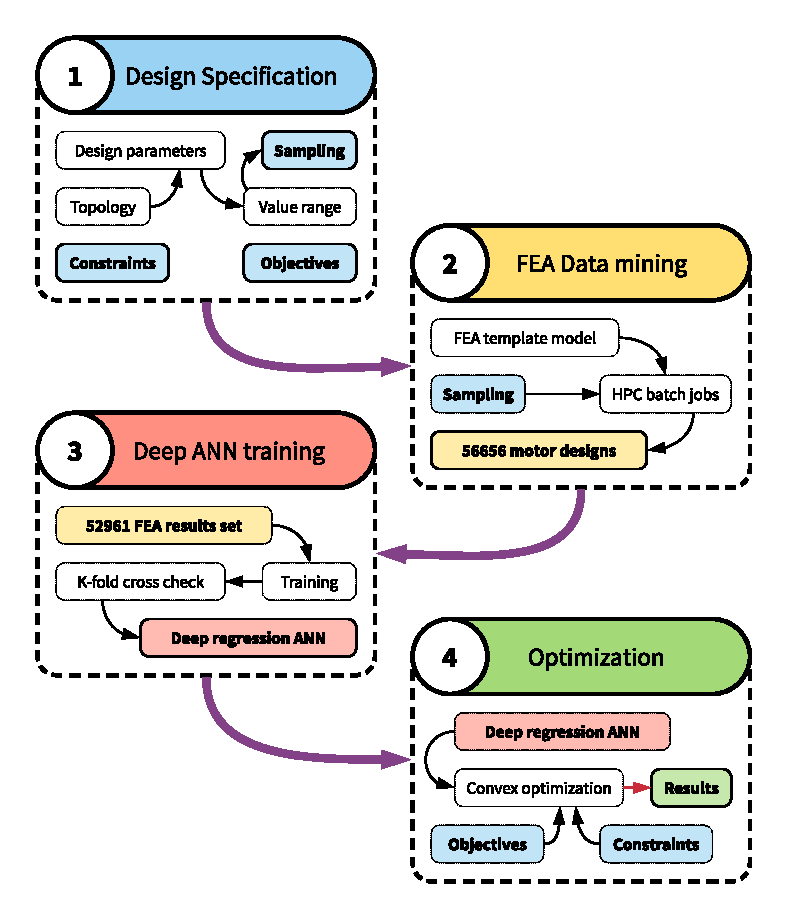
\includegraphics[width=4.5in]{chap4/images2/LFSM_design_process.pdf}
            \caption{Flowchart of the RSM motor design process adapted for \acs{LFSM}.}
            \label{fig:chapter/rsm/LFSM/design process}
        \end{figure*}
    
    
        % -----------------------------------------------------------------------------------
        % --- NEW SUB SECTION --- NEW SUB SECTION --- NEW SUB SECTION --- NEW SUB SECTION --- 
        % -----------------------------------------------------------------------------------
        \subsection{Specifications \& Samplings}    \label{Chapter:RSM/LFSM/spec}
        
        
            This work investigate and optimize tubular linear 6 slot/7 pole machine with the dimensions presented in Fig.\,\ref{fig:chapter/rsm/LFSM/structure} and \,\ref{fig:chapter/rsm/LFSM/machine design}. With consideration to the dimensions and ratios of the desired motor design, the structural design factors and their range are summarized in Table\,\ref{table:chap/rsm/LFSM/design range}. 
            
            
            The magnet, conductor and \acs{SMC} core assembly as a whole body is treated as the mover, and the \acs{SMC} track with trapezoid teeth is treated as the stator. The stator core inner radius $r_{si}$ and the mover-stator air gap $h_G$ are fixed at $2\mathrm{mm}$ and $1.2\mathrm{mm}$, respectively. With an effective stator pocket of $4\,\mathrm{mm}$ in diameter, the structural support has a place to be added later on. For the ease of manufacturing, there needs to be a reasonable amount of air gap between the stator and mover such as $1.2\mathrm{mm}$, which comes from our past experience building tubular longitudinal synchronous motor. Physically, this air gap will include non-magnetic support structures as well as mechanical clearance. Note that in the data collection process, the motor length $L_S$ and stroke length $L_{stroke}$ are not yet determined. Instead, the length of each repeat 6 slot/7 pole unit $L_{repeat}$ is iterated upon. To simplify the model the tooth angle $\theta$ is set to be the value of $\arctan{1/2}$, which makes the width of each tooth extension precisely half the height of the tooth.
            
            
            Table\,\ref{table:chap/rsm/LFSM/sampling levels} shows incremental sampling steps for the structural design factors. From the sampling steps, a design grid of $46656$ cases are generated. Additionally, another $10000$ cases constructed by input variables created with random values within Table\,\ref{table:chap/rsm/LFSM/design range} range were added to help generalize the entire continuous design space better. In total, there were $56656$ independent motor designs to have their average thrust, maximum thrust, and cogging profile predicted by \acs{FEA}.
            
            
            \begin{table}[!ht]
                \renewcommand{\arraystretch}{1.2}
                \caption{Summary of the \acs{LFSM} motor parameter ranges}
                \label{table:chap/rsm/LFSM/design range}
                \centering
                \begin{tabular}{@{}llr@{}}
                \hline
                \bfseries Parameter & \bfseries Description & \bfseries Values\\
                \hline
                    $\alpha$	    & Ratio of $w_M$ over $L_{KC}$              &	$0.1-0.4$\\ 
                    $\beta$	        & Ratio of $w_C$ over $w_S$		            &	$0.4-0.9$\\ 
                    $\gamma$	    & Ratio of $h_{CM}$ over $h_C$			    &	$0.6-0.9$\\ 
                    $\delta$	    & Ratio of $w_R$ or $L_{KS}$		        &	$0.1-0.2$\\ 
                    $\epsilon$	    & Ratio of $h_{R1}$ or $h_{R2}$		        &	$0.4-0.6$\\ 
                    $r_{si}$	    & Inner radius of SMC stator core 	        &	$2\,\mathrm{mm}$\\ 
                    $r_{so}$	    & Outer radius of SMC stator core 			&	$4-10\,\mathrm{mm}$\\ 
                    $h_C$           & Thickness of the mover assembly           &	$5-30\,\mathrm{mm}$\\ 
                    $h_G$	        & Mover-stator air gap 					    &	$1.2\,\mathrm{mm}$\\ 
                    $L_{repeat}$	& Length of each 6 slot/7 pole unit 		&	$50-90\,\mathrm{mm}$\\ 
                    $\theta$	    & Stator tooth angle 		                &	$\arctan(1/2)$\\ 
                    $N_C$	        & Number of armature slots 		            &	    $6$\\ 
                    $N_S$	        & Number of mover pole 		                &	$\geq 7$\\ 
                \hline
                \end{tabular}
            \end{table}
            
            
            \begin{table}[!ht]
                \renewcommand{\arraystretch}{1.2}
                \caption{Summary of the \acs{LFSM} motor parameter sampling levels}
                \label{table:chap/rsm/LFSM/sampling levels}
                \centering
                \begin{tabular}{@{}l r r r r r r r@{}}
                \hline
                \bfseries Params & \bfseries Level 1 & \bfseries Level 2 & \bfseries Level 3 & \bfseries Level 4 & \bfseries Level 5 & \bfseries Level 6 & \bfseries Unit \\
                \hline
                    $\alpha$     & 0.1     & 0.2  & 0.3 & 0.4 & -   & -   &               \\
                    $\beta$      & 0.4     & 0.5  & 0.6 & 0.7 & 0.8 & 0.9 &               \\
                    $\gamma$     & 0.6     & 0.7  & 0.8 & 0.9 & -   & -   &               \\
                    $\delta$     & 0.1     & 0.15 & 0.2 & -   & -   & -   &               \\
                    $\epsilon$   & 0.4     & 0.5  & 0.6 & -   & -   & -   &               \\
                    $r_{so}$     & 4       & 7    & 10  & -   & -   & -   &               \\
                    $h_C$        & 5       & 10   & 15  & 20  & 25  & 30  & $\mathrm{mm}$ \\
                    $L_{repeat}$ & 50      & 70   & 10  & -   & -   & -   & $\mathrm{mm}$
                    \\
                \hline
                \end{tabular}
            \end{table}
                    
        
        % -----------------------------------------------------------------------------------
        % --- NEW SUB SECTION --- NEW SUB SECTION --- NEW SUB SECTION --- NEW SUB SECTION --- 
        % -----------------------------------------------------------------------------------
        \subsection{\acs{FEA} data mining}          \label{Chapter:RSM/LFSM/data mining}
        
        
            Due to the complex flux pattern inherent to the doubly-salient structure in the mover assembly, estimating average thrust of a design requires knowledge of the maximum achievable forces at different stroke positions.

            The 6 slot/7 pole machine was modelled in ANSYS MAPDL to measure the force generated on the secondary, as shown in Fig.\,\ref{fig:chapter/rsm/LFSM/FEA}. The 2D axis-symmetric model implemented in ANSYS  $19.2$ uses a mapped mesh for the motor parts and a free mesh for the transition regions such as the air gap and the free space surrounding the structure. Periodic boundary conditions were not applied at each end of the armature repeat unit along the $\hat{z}$ direction. This setup therefore does not ignore end effects. If we were to apply the periodic boundary condition at each end of the armature, and at the same time experiment with a non zero secondary tooth angle, the ANSYS MAPDL becomes significantly more prone to execution errors. Instead the simulation setup adds 3 extra teeth on each end of the secondary. As the result all simulation test cases has exactly 6 armature slots, and 13 teeth.
            

            The \acs{SMC} parts and magnets are made out of Sintex \acs{SMC} prototype materials and K$\&$J Magnetics Grade N45SH, respectively. The non-linear $\mathrm{B-H}$ relationship of the \acs{SMC} material is also fully captured in the FEA model. This setup will be crucial to the design optimization process, where many different design configurations need to be tested.
            
            
            \begin{figure*}[!ht]
                \centering
                \subfloat[\label{fig:chapter/rsm/LFSM/FEA/position 1} \acs{FEA} mesh view of \acs{LFSM} for the beginning position]{
                    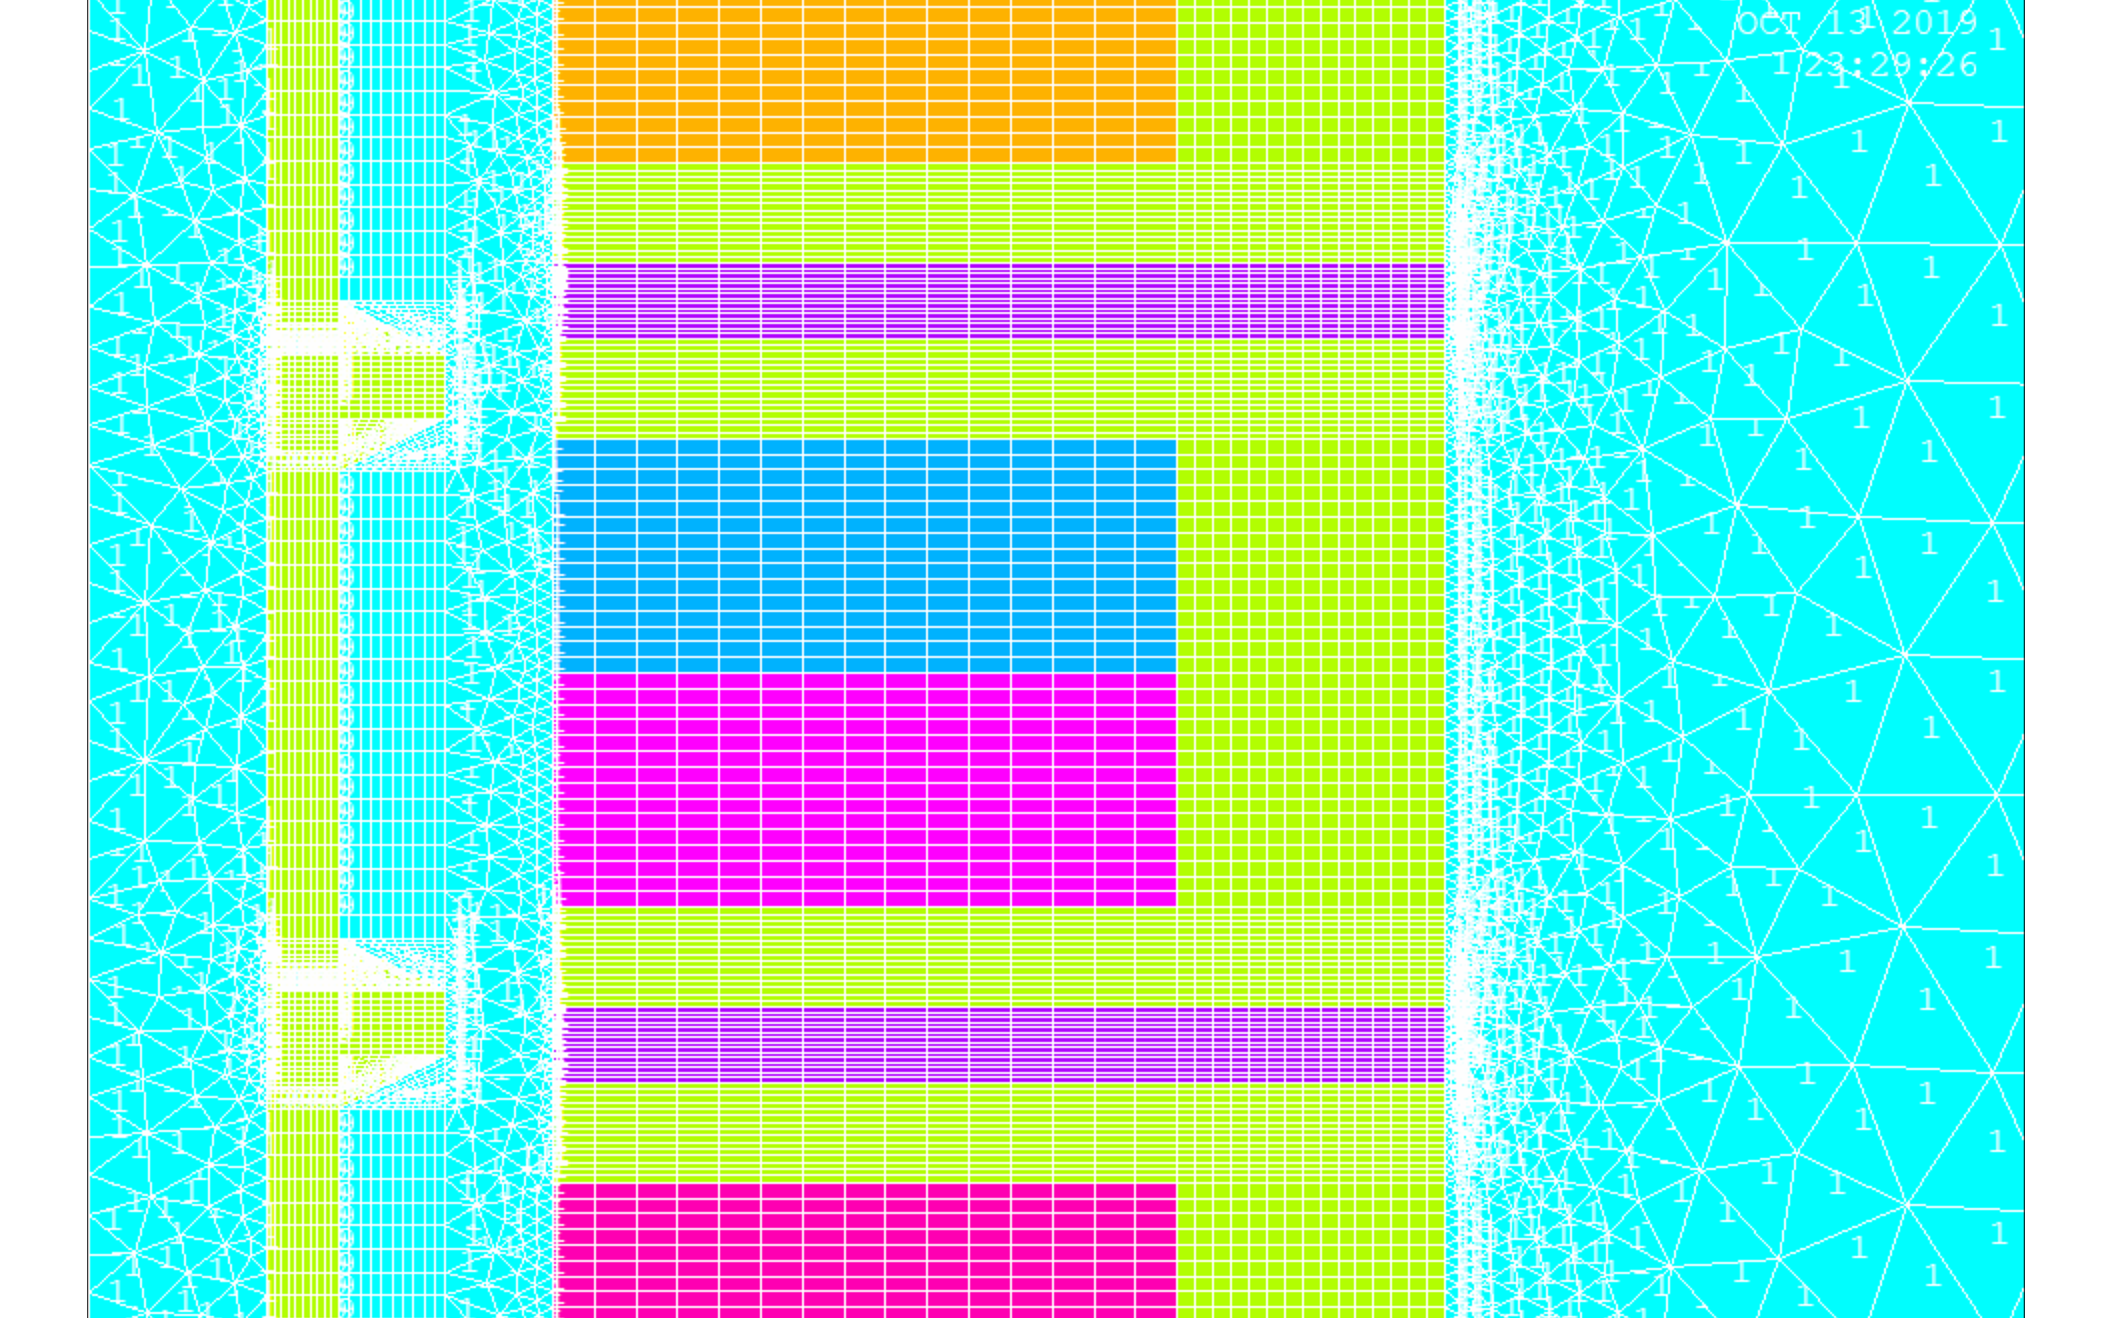
\includegraphics[width=0.6\textwidth]{chap4/images2/FEA_position_1.png}
                }
                \\
                \subfloat[\label{fig:chapter/rsm/LFSM/FEA/position 10} \acs{FEA} mesh view of \acs{LFSM} for the middle position]{
                    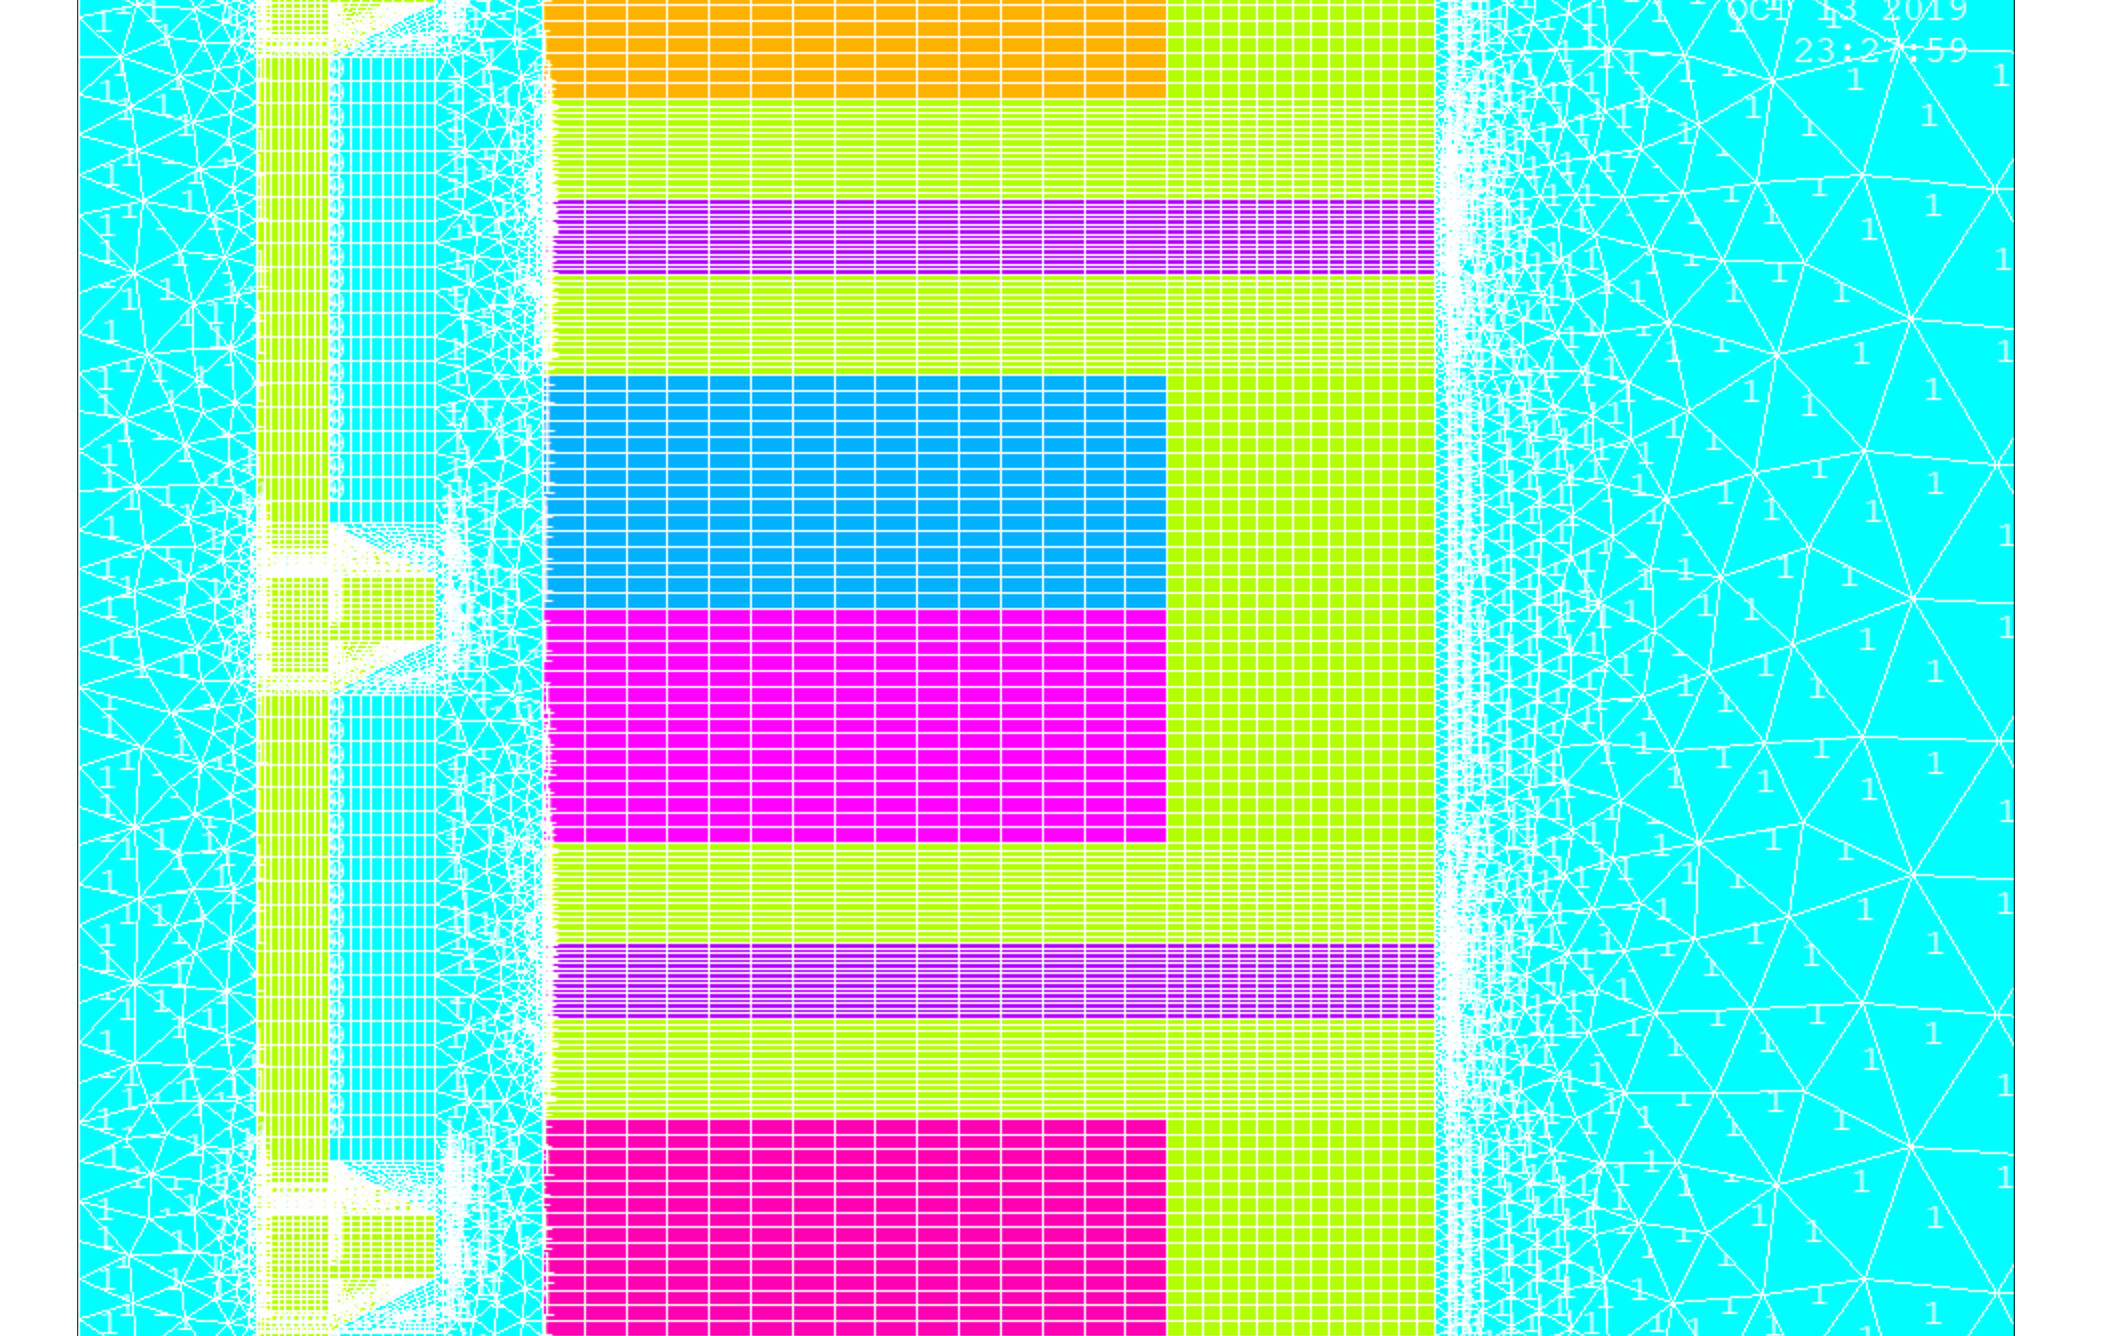
\includegraphics[width=0.6\textwidth]{chap4/images2/FEA_position_10.png}
                }
                \caption{ 
                    \label{fig:chapter/rsm/LFSM/FEA} FEA setup for obtaining the resultant thrust given a stroke position, a 3-phase current angle, a set of design parameters, and the fixed input power. The graphics cropped from ANSYS MAPDL $19.2$ shows the \acs{SMC} material in green, the free space in blue, the axial permanent magnet rings in dark purple, and the coil phases.
                }
            \end{figure*}
            
            
            The base modelling script was constructed with the intention to allow for easy modification of the input parameters summarized in Table\,\ref{table:chap/rsm/LFSM/design range}. For the $56656$ motor designs, we need to determine the cogging force, average thrust, and peak thrust at $1500\,\mathrm{W}$ input power. We take force measurements at $20$ equally spaced stroke positions and $42$ current angle offsets. Since the the mesh of each simulation can be reused for all the different current angle offsets, only the different stroke positions require re-meshing. In total, there are $1133120$ input files which represent all the unique permutations of all motor design dimensions, stroke positions, and current angle offsets. Additionally, each input files contain an extra simulation at null applied current to learn about the cogging force at the various stroke positions. 
            
            
            We sent these $1133120$ input files to the high performance computing (HPC) infrastructure owned by the New Zealand eScience Infastructure (NeSI) for execution in parallel batches. Each input file is estimated to take $22$ minutes on a two-core Intel CPU with $3\,\mathrm{GBs}$ of RAM. Given that the HPC facility allows for any user to execute $1000$ jobs in parallel, this consumed $415506$ CPU hours, and took approximately $416$ hours to complete. All verbose output of jobs were collected and doubled checked for errors and warnings, totalling $435\,\mathrm{GBs}$ of raw data in text format. The necessary information was then reduced back to $52961$ fully captured motor designs in CSV format, demonstrating a high success rate of more than $93.5\,\%$. The computed thrust output by FEA batches was later further processed and refined into peak to peak cogging force $F_{\Delta cogging}$, average thrust $\overline{F}$, and peak thrust $F_{peak}$ for use in training the neural network.
            
            
            One additional advantage of having the data ready ahead of the optimization process is that the available data, though limited, can still provide valuable insights into identifying the principal design parameters. To investigate these hidden relationships, we plot a heat map in Fig.\,\ref{fig:chap/rsm/LFSM/data mining/heat map}. We can learn a number of useful relationships from this heat map:
            
            
            \begin{itemize}
                \item $\alpha$ ratio can improve the average and peak thrust at the cost of more peak to peak cogging $F_{\Delta cogging}$,
                \item $r_{so}$ also improve average and peak thrust without adding more cogging, however, this will inherently add more mass,
                \item Low $\beta$ is more preferable,
                \item Surprisingly, stator tooth design factors such as $\epsilon$ and $\delta$ has very little influence on the motor performance, even on the peak to peak cogging $F_{\Delta cogging}$
            \end{itemize}
            
            
            \begin{figure}
                \centering
                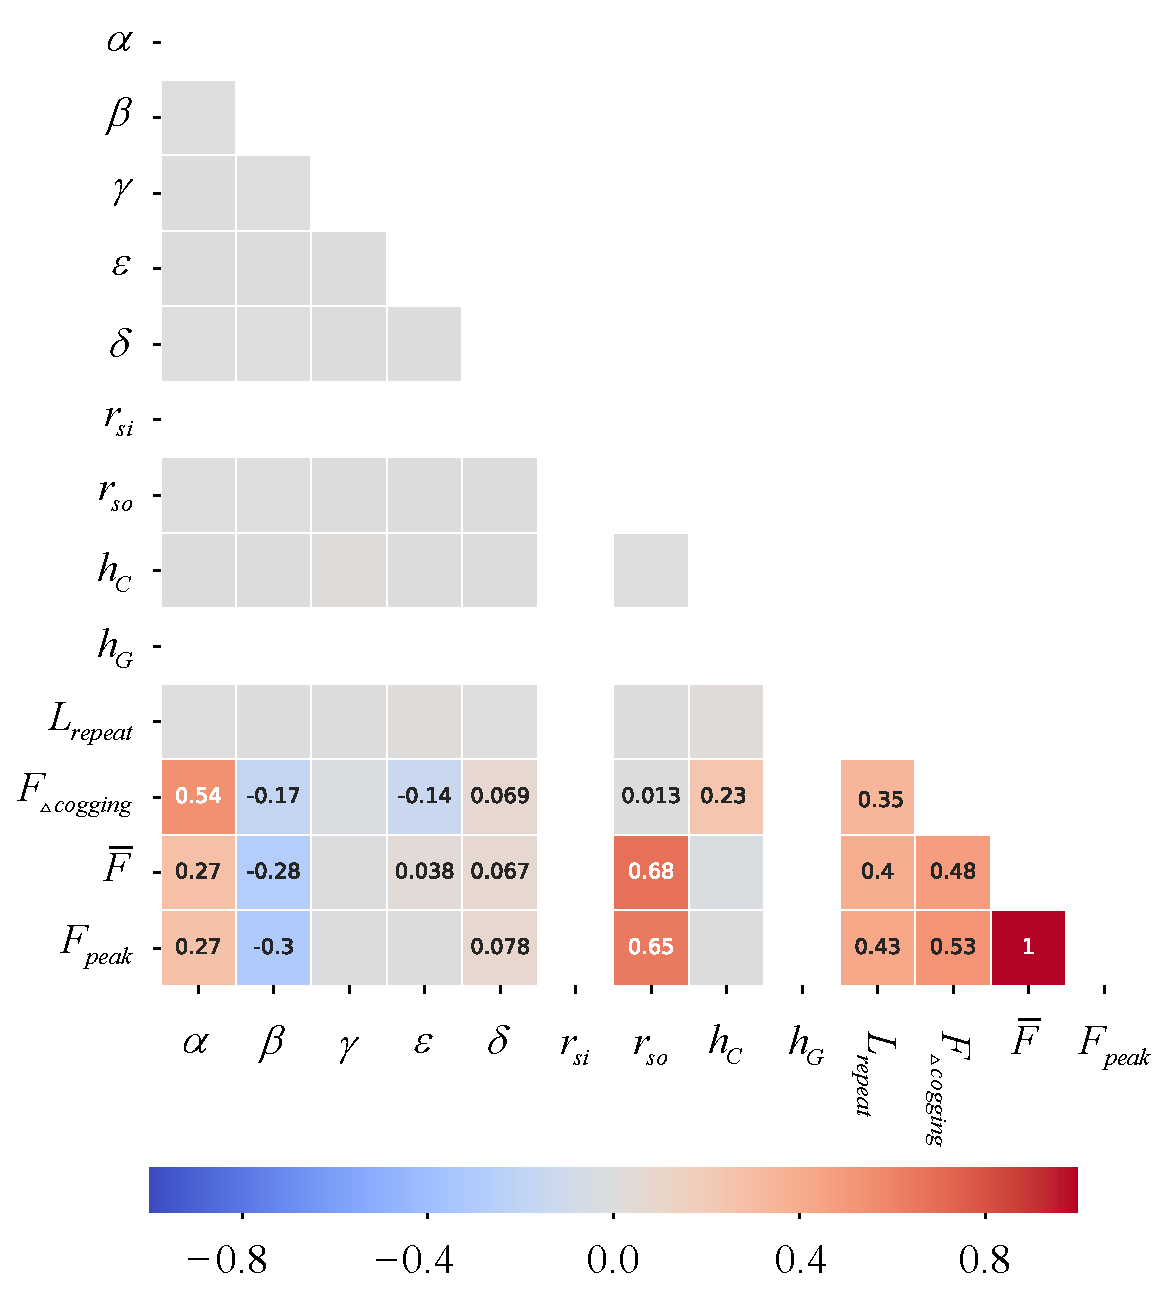
\includegraphics[width=5in, trim=0 0 0 129mm, clip]{chap4/images2/heatmap.pdf}
                \caption{Heat map which depicts the relationship between different input and output variables of the motor design data set obtained in the \acs{FEA} data mining step for \acsp{LFSM}. Red and blue on this scale mean positively and negatively correlated. Small values are hidden.}
                \label{fig:chap/rsm/LFSM/data mining/heat map}
            \end{figure}
        
        
        % -----------------------------------------------------------------------------------
        % --- NEW SUB SECTION --- NEW SUB SECTION --- NEW SUB SECTION --- NEW SUB SECTION --- 
        % -----------------------------------------------------------------------------------
        \subsection{Deep regression ANN training}   \label{Chapter:RSM/LFSM/ANN training}
        
        
            The data set provides both the continuous input variables (structural design factors), and the continuous output variable (thrust characteristics at a given power), which classify our application as a supervised and regression type of machine learning problem. The ANN model was implemented in Keras and Tensorflow:

            
            \begin{itemize}
                \item $8$ structural parameters and the input power are regarded as the Input Layer: $\alpha$, $\beta$, $\gamma$, $\epsilon$, $\delta$, $r_{so}$, $h_G$, and $L_{repeat}$,
                \item $3$ performance outputs are regarded as the Output Layer: $F_{\Delta cogging}$, $\overline{F}$, and $F_{peak}$,
                \item $\mathrm{Adam}$ optimizer is used for ANN training,
                \item $6$ hidden layers of $256-512-512-512-512-512$ of densely connected nodes,
                \item Rectified linear unit (ReLU) activation function is used
for the input and hidden layer,
                \item Linear activation function is used for the output layer,
                \item The error to optimize for is \acs{MSE},
                \item The training and validation split chosen at random for each of the three models are: $70\%-30\%$, $75\%-25\%$, and $80\%-20\%$,
                \item The final \acs{ANN} model is ensembled from the average of three models above.
            \end{itemize}


            After 500 training iterations, the model was shown to have a \acf{MAPE} of under $2.41\,\%$. Fig.\,\ref{fig:chapter/rsm/LFSM/training result} is showing that he training and validation errors were similar, which means the deep regression model is not over-fitted to the training data set.
            
            
            \begin{figure*}[!ht]
                \centering
                \subfloat[$70\%-30\%$ split model
                ]{
                    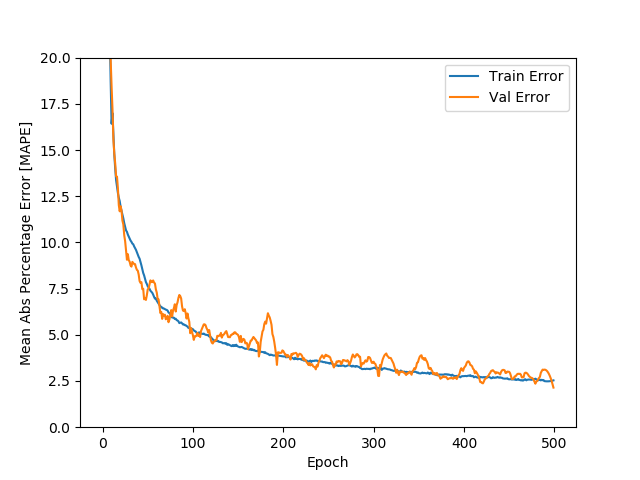
\includegraphics[width=0.5\textwidth]{chap4/images2/MAPE_MSE_6_70-30_SPLIT.png}
                    \label{fig:chapter/rsm/LFSM/training result/MAPE_70_30}
                }
                \subfloat[$75\%-25\%$ split model
                ]{
                    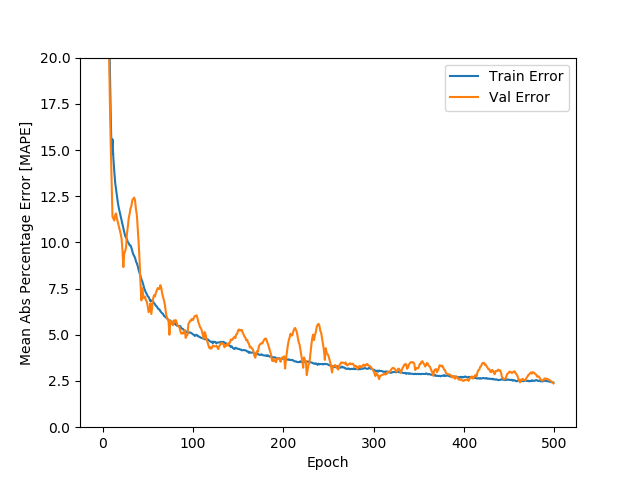
\includegraphics[width=0.5\textwidth]{chap4/images2/MAPE_MSE_6_75-25_SPLIT.png}
                    \label{fig:chapter/rsm/LFSM/training result/MAPE_75_25}
                }
                \\
                \subfloat[$80\%-20\%$ split model
                ]{
                    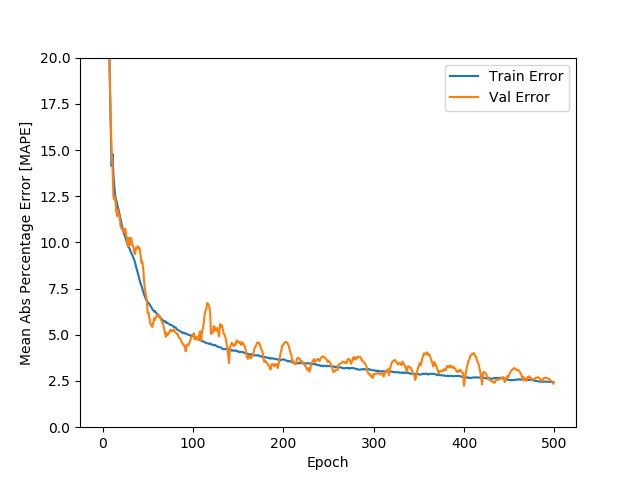
\includegraphics[width=0.5\textwidth]{chap4/images2/MAPE_MSE_6_80-20_SPLIT.png}
                    \label{fig:chapter/rsm/LFSM/training result/MAPE_80_20}
                }
                \caption{
                    Error produced by the deep learning ANN model to represent \acsp{LFSM} vs. iterations for the training data (blue) and validation data (orange). The \acs{MAPE} is plotted for the training process of (a) $70\%-30\%$, (b) $75\%-25\%$, and (c) $80\%-20\%$ models, respectively.
                }   \label{fig:chapter/rsm/LFSM/training result}
            \end{figure*}
        
        
        % -----------------------------------------------------------------------------------
        % --- NEW SUB SECTION --- NEW SUB SECTION --- NEW SUB SECTION --- NEW SUB SECTION --- 
        % -----------------------------------------------------------------------------------
        \subsection{Optimization}                   \label{Chapter:RSM/LFSM/Optimization}
    
    
    % ===================================================================================================
    % === NEW SECTION === NEW SECTION === NEW SECTION === NEW SECTION === NEW SECTION === NEW SECTION ===
    % ===================================================================================================
    \section{Application to \ac{LTFM}}               \label{Chapter:RSM/LTFM}
    
        
        % -----------------------------------------------------------------------------------
        % --- NEW SUB SECTION --- NEW SUB SECTION --- NEW SUB SECTION --- NEW SUB SECTION --- 
        % -----------------------------------------------------------------------------------
        \subsection{Specifications \& Samplings}    \label{Chapter:RSM/LTFM/spec}
        
        
        % -----------------------------------------------------------------------------------
        % --- NEW SUB SECTION --- NEW SUB SECTION --- NEW SUB SECTION --- NEW SUB SECTION --- 
        % -----------------------------------------------------------------------------------
        \subsection{\acs{FEA} data mining}          \label{Chapter:RSM/LTFM/data mining}
        
        
        % -----------------------------------------------------------------------------------
        % --- NEW SUB SECTION --- NEW SUB SECTION --- NEW SUB SECTION --- NEW SUB SECTION --- 
        % -----------------------------------------------------------------------------------
        \subsection{Deep regression ANN training}   \label{Chapter:RSM/LTFM/ANN training}
        
        
        % -----------------------------------------------------------------------------------
        % --- NEW SUB SECTION --- NEW SUB SECTION --- NEW SUB SECTION --- NEW SUB SECTION --- 
        % -----------------------------------------------------------------------------------
        \subsection{Optimization}                   \label{Chapter:RSM/LTFM/Optimization}
    
    
    
    % ===================================================================================================
    % === NEW SECTION === NEW SECTION === NEW SECTION === NEW SECTION === NEW SECTION === NEW SECTION ===
    % ===================================================================================================
    \section{Discussion}                            \label{Chapter:RSM/discussion}
    
